%% ---------------------------------------------------------------------------
%% IJACSA (The Science and Information Organization) paper format.
%% Preamble, header and footer follow the official SAI LaTeX template
%% (SAI_Paper_Format_Latex: IEEEtran, conference, US letter).
%%
%% Two versions are built from this single source:
%%   54_ijacsa.tex        anonymised manuscript for double-blind review (default)
%%   54_ijacsa_final.tex  camera-ready version: defines \FINALVERSION and
%%                        \input's this file, restoring authors, affiliation,
%%                        corresponding author, repository link and funding.
%% Figures are read from ../Images (the same files the plotting scripts write).
%% ---------------------------------------------------------------------------
\documentclass[conference, letterpaper]{IEEEtran}

\newif\ifblind
\ifdefined\FINALVERSION \blindfalse \else \blindtrue \fi

\ifCLASSINFOpdf
   \usepackage[pdftex]{graphicx}
\else
\fi
\graphicspath{{../Images/}}
\hyphenation{op-tical net-works semi-conduc-tor}

\usepackage[cmex10]{amsmath}
\usepackage{color}
% The SAI template also loads flushend; together with \balance it breaks the
% last page (columns and footer overlap), so only balance is used here.
\usepackage{fancyhdr}
\usepackage{subcaption}
\usepackage{balance}
\captionsetup[table]{justification=centering, labelsep=period, font={footnotesize,sc}}
\captionsetup[figure]{justification=centering, labelsep=period, font={footnotesize}}
\usepackage{booktabs}
\usepackage{threeparttable}
\usepackage{multirow}
\usepackage{array}
\usepackage{url}

% Float placement: lets figures and tables sit at the top or bottom of the
% column that cites them instead of drifting to later pages. Margins, column
% widths and fonts of the template are unchanged.
\renewcommand{\topfraction}{0.9}
\renewcommand{\bottomfraction}{0.6}
\renewcommand{\textfraction}{0.1}
\renewcommand{\floatpagefraction}{0.8}
\renewcommand{\dbltopfraction}{0.9}
\renewcommand{\dblfloatpagefraction}{0.8}
\setcounter{topnumber}{3}
\setcounter{bottomnumber}{2}
\setcounter{totalnumber}{5}
\setcounter{dbltopnumber}{3}

% Header and footer of the SAI template
\renewcommand{\thispagestyle}[2]{}
\fancypagestyle{plain}{
        \fancyhead{}
        \fancyhead[C]{first page center header}
        \fancyfoot{}
        \fancyfoot[C]{first page center footer}
}
\pagestyle{fancy}
\headheight 20pt
\footskip 20pt
\rhead{}
\setcounter{page}{1}
\fancyhead[R]{\textit{(IJACSA) International Journal of Advanced Computer Science and Applications, \\ Vol. XXX, No. XXX, 2026}}
\renewcommand{\headrulewidth}{0pt}
\fancyfoot[C]{www.ijacsa.thesai.org}
\renewcommand{\footrulewidth}{0.5pt}
\fancyfoot[R]{\thepage \  $|$ P a g e }

% Links without coloured boxes; PDF metadata carries no author data in the
% blind version
\usepackage[hidelinks]{hyperref}
\ifblind
\hypersetup{pdftitle={Semantic Search of Scientific Abstracts through Hierarchical Navigable Small World Indexing in Vector Databases},
            pdfauthor={}, pdfsubject={}, pdfkeywords={}, pdfcreator={}}
\else
\hypersetup{pdftitle={Semantic Search of Scientific Abstracts through Hierarchical Navigable Small World Indexing in Vector Databases},
            pdfauthor={Santiago Callocondo-Garay, Piero Mejia-Ramos, Antonio Arroyo-Paz}}
\fi

\newcommand{\efc}{\textit{ef\_construction}}
\newcommand{\efs}{\textit{ef\_search}}
\newcommand{\doi}[1]{doi:~\href{https://doi.org/#1}{\nolinkurl{#1}}}
\newcommand{\ijacsa}{\textit{International Journal of Advanced Computer Science and Applications}}

\begin{document}

\title{Semantic Search of Scientific Abstracts through Hierarchical Navigable Small World Indexing in Vector Databases}

\ifblind
\author{\IEEEauthorblockN{Anonymous Authors}
\IEEEauthorblockA{Affiliation withheld for double-blind review}}
\else
\author{\IEEEauthorblockN{Santiago Callocondo-Garay$^{*}$, Piero Mejia-Ramos, Antonio Arroyo-Paz}
\IEEEauthorblockA{Escuela Profesional de Ingenier\'{\i}a de Sistemas, Universidad Nacional de San Agust\'{\i}n, Arequipa, Per\'u}}
\fi

\maketitle

\ifblind\else
\renewcommand{\thefootnote}{\fnsymbol{footnote}}
\footnotetext[1]{Corresponding author (scallocondo@unsa.edu.pe)}
\fi

% Abstract: no symbols, special characters or mathematics (SAI template rule)
\begin{abstract}
Approximate nearest neighbor search makes semantic retrieval practical on large document collections, and Hierarchical Navigable Small World (HNSW) graphs are its most widely used index. This study evaluates HNSW, as implemented in the FAISS library, for semantic search over 48,018 arXiv abstracts, using 1,000 held-out abstracts as queries. A controlled grid over the number of links per node, the construction candidate list and the search candidate list was built five times per configuration to measure how faithfully the index reproduces exact search, together with single-thread latency, build time and memory, and a reference configuration was selected with an explicit rule. The number of links per node dominates fidelity, whereas quadrupling the construction candidate list roughly triples build time for a mean recall gain of at most 0.005. The reference configuration reaches a recall at rank 10 of 0.997 with SciBERT and 0.992 with E5-large in under one millisecond per query. Index fidelity, however, says little about retrieval quality. When each title is used to retrieve its own abstract, exact search places it in the top 10 for 17 percent of titles with SciBERT and 95 percent with E5-large, while all six embedding models evaluated keep a fidelity between 0.986 and 0.998. A factorial comparison of models attributes this gap to the training objective rather than to the scientific domain. Query encoding accounts for more than 98 percent of end-to-end latency. HNSW is faster than inverted-file, product-quantization and ball-tree indexes at high recall, and it scales sublinearly to 500,000 vectors, where it is 32 times faster than exact search.
\end{abstract}

\begin{IEEEkeywords}
Approximate nearest neighbor search; hierarchical navigable small world; vector databases; semantic search; text embeddings; scientific document retrieval; FAISS; information retrieval
\end{IEEEkeywords}

\IEEEpeerreviewmaketitle

% =====================================================================
\section{Introduction}
% =====================================================================

Scientific literature grows faster than keyword search can keep up with. As of May 2026, arXiv holds more than 2.6 million papers \cite{arxivstats} and PubMed indexes more than 38 million biomedical records \cite{pubmed}. Two abstracts can describe the same idea without sharing a single term, a vocabulary mismatch that keyword search only partly bridges, for example by expanding queries with word embeddings and ontologies \cite{rastogi2021}. Semantic search instead represents each document as a dense vector, or \textit{embedding}, that captures similarity beyond the literal vocabulary \cite{reimers2019,ajallouda2025}. The cost reappears at query time: finding the exact nearest neighbors means comparing the query with every vector, an $O(N \cdot d)$ cost that grows linearly with the collection. Large-scale retrieval therefore relies on approximate nearest-neighbor (ANN) search, which gives up a small amount of accuracy for much faster answers \cite{mathur2024}.

Among ANN methods, Hierarchical Navigable Small World (HNSW) graphs \cite{malkov2020} have become the de facto standard. Inspired by small-world networks \cite{watts1998}, HNSW organizes the vectors in a multi-layer graph with logarithmic query complexity and recalls above 97\,\% on standard benchmarks \cite{malkov2020}, and it is the primary index of libraries and systems such as FAISS \cite{johnson2021} and Milvus \cite{wang2021}. These systems now sit behind many retrieval-augmented generation (RAG) pipelines \cite{lewis2020}, including recent applications to document question answering \cite{muludi2024}, software-development queries \cite{huan2024}, court rulings \cite{ibrihich2026} and image retrieval \cite{shuo2024}. The performance of HNSW, however, is not constant. It depends on the number of links per node $M$ and on the candidate list used while building, \efc{}, which set the balance between construction cost and recall \cite{zhao2025}, and on the candidate list used at query time, \efs{}, which sets the balance between recall and latency. Studies of these trade-offs, and of the similarity metric, mostly use general-purpose corpora and question-answering data \cite{elkiran2025,rajpurkar2016}.

Scientific abstracts are a harder setting: the vocabulary is dense and specialized, and topics are unevenly distributed. They also raise a question that index benchmarks usually leave aside. An index is evaluated against exact search in the same vector space, so a high recall says that the index is faithful to the embedding model, not that the documents it returns are relevant. Whether a scientific model such as SciBERT \cite{beltagy2019} or a general retrieval model such as E5 \cite{wang2022} serves a search engine better is a separate question, and the two models differ both in domain and in training objective.

This work evaluates HNSW, as implemented in FAISS, for semantic search over arXiv abstracts. Its contributions are empirical:
\begin{itemize}
\item A controlled grid over $M$, \efc{} and \efs{} with repeated builds, single-thread latency, build time and memory, and an explicit rule to select a configuration instead of ranking by recall alone.
\item A separation of index fidelity from retrieval quality through a known-item task, in which titles are used to find their own abstracts, and a factorial set of six models that separates the scientific domain from the training objective.
\item End-to-end latency, including query encoding, and a comparison of HNSW with inverted-file, product-quantization and tree indexes on the same queries.
\item Scalability measured at constant recall up to 500,000 vectors, with fitted growth rates.
\end{itemize}

The rest of the paper is organized as follows. Section~\ref{sec:related} reviews work on ANN indexes, vector databases and embedding models. Section~\ref{sec:method} describes the data, the models, the experimental grid and the evaluation protocol. Section~\ref{sec:results} reports the results, Section~\ref{sec:discussion} discusses their implications and limitations, and Section~\ref{sec:conclusion} concludes.

% =====================================================================
\section{Related Work}
\label{sec:related}
% =====================================================================

\subsection{Approximate Nearest-Neighbor Indexes}

ANN algorithms address the cost of exact $k$-nearest-neighbor search in high-dimensional spaces. Mathur and Chhabra \cite{mathur2024} group them into four families (exhaustive search, trees, quantization and graphs) and find graph-based methods the most competitive as dimensionality grows; the ANN-Benchmarks suite reaches similar conclusions on standard datasets \cite{aumuller2020}. HNSW \cite{malkov2020} belongs to the graph family: its upper layers provide long, sparse hops and its base layer refines the local search. Iwasaki and Miyazaki \cite{iwasaki2018} adjust the in-degree and out-degree of each node of a nearest-neighbor graph, removing redundant edges without losing accuracy, and Zhao et al.~\cite{zhao2023} guide each insertion with a lightweight search based on locality-sensitive hashing (LSH-APG), so that the graph can be maintained incrementally as the collection grows.

The weak point of HNSW is construction rather than querying: each insertion triggers several multi-layer searches and many distance computations \cite{zhao2025}. Zhao et al.~\cite{zhao2025} propose H-DMax, which prunes distant neighbors hierarchically with a factor $\lambda$; on SIFT1M, $\lambda=1.10$ speeds up construction by $1.10\times$ with a Recall@10 loss of 0.27 points, and $\lambda=1.20$ reaches $1.27\times$ at a loss of 1.03 points. Product quantization \cite{jegou2011} follows another route and compresses the vectors into short codes; in the same study, HNSW with product quantization builds $3.6\times$ faster than plain HNSW, but its Recall@10 falls to 85\,\% \cite{zhao2025}. Optimized product quantization (OPQ) rotates the space before quantizing to reduce that loss \cite{ge2014}. In image retrieval, a recent systematic review of large-scale indexing covers inverted-file, product-quantization and hashing schemes and identifies scalability and real-time processing as persistent challenges \cite{saouabe2024}.

\subsection{Vector Databases and Retrieval Pipelines}

FAISS \cite{johnson2021} and Milvus \cite{wang2021} are common infrastructure for HNSW and other indexes. Milvus supports cosine, inner product and $L_2$ distance and underlies many RAG pipelines \cite{lewis2020}. On it, Elkiran and Rasheed \cite{elkiran2025} compared the three metrics with 3,072-dimensional OpenAI embeddings on SQuAD \cite{rajpurkar2016}: cosine and inner product reached a Recall@10 of 0.909--0.925 and an MRR of 0.781--0.793, while unnormalized $L_2$ reached 0.373 and 0.116. On unit vectors the three metrics rank neighbors identically, so normalization is what matters.

Applied systems show how vector search is usually deployed. Muludi et al.~\cite{muludi2024} answer questions over documents with a RAG pipeline that retrieves passages through FAISS, and Huan and Zhou \cite{huan2024} build a FAISS vector store to retrieve answers to web-development questions. Ibrihich et al.~\cite{ibrihich2026} keep multilingual E5 embeddings of court rulings in an exact FAISS inner-product index and fuse its ranking with BM25, and Shuo et al.~\cite{shuo2024} store convolutional image features in an inverted-file index of Milvus, noting that approximate search may not return the exact neighbors in exchange for speed. These studies evaluate the end task, such as answer quality or retrieval precision, with one index configuration, and do not separate the error of the approximate index from that of the embedding model.

\subsection{Embedding Models for Scientific Text}

SciBERT \cite{beltagy2019} adapts BERT \cite{devlin2019} to scientific vocabulary but is not trained for similarity, and the quality of sentence vectors taken from a pre-trained BERT varies with the layer they are extracted from \cite{alsuhaibani2023}. SPECTER2 \cite{singh2023} and SciNCL \cite{ostendorff2022} learn document similarity from citations, and E5 \cite{wang2022} learns it from large sets of query--passage pairs. A recent review of sentence embedding models found that BERT and RoBERTa underperformed on retrieval \cite{ajallouda2025}, and in a comparison of ten multilingual models for Arabic retrieval, E5 reached the highest recall, above 0.90 at rank 10 \cite{abdelazim2023}. Relevance benchmarks such as BEIR \cite{thakur2021} evaluate these models with exact search, while ANN benchmarks evaluate indexes on fixed vectors \cite{aumuller2020}. We found no study that measures HNSW parameters on scientific abstracts and, at the same time, separates the fidelity of the index from the retrieval quality of the model that feeds it.

% =====================================================================
\section{Methodology}
\label{sec:method}
% =====================================================================

Fig.~\ref{fig:pipeline} summarizes the pipeline. Embeddings are computed once on a GPU; all indexing, search and timing runs on a CPU, from frozen vectors and frozen lists of document identifiers.

\begin{figure}[!tb]
\centering
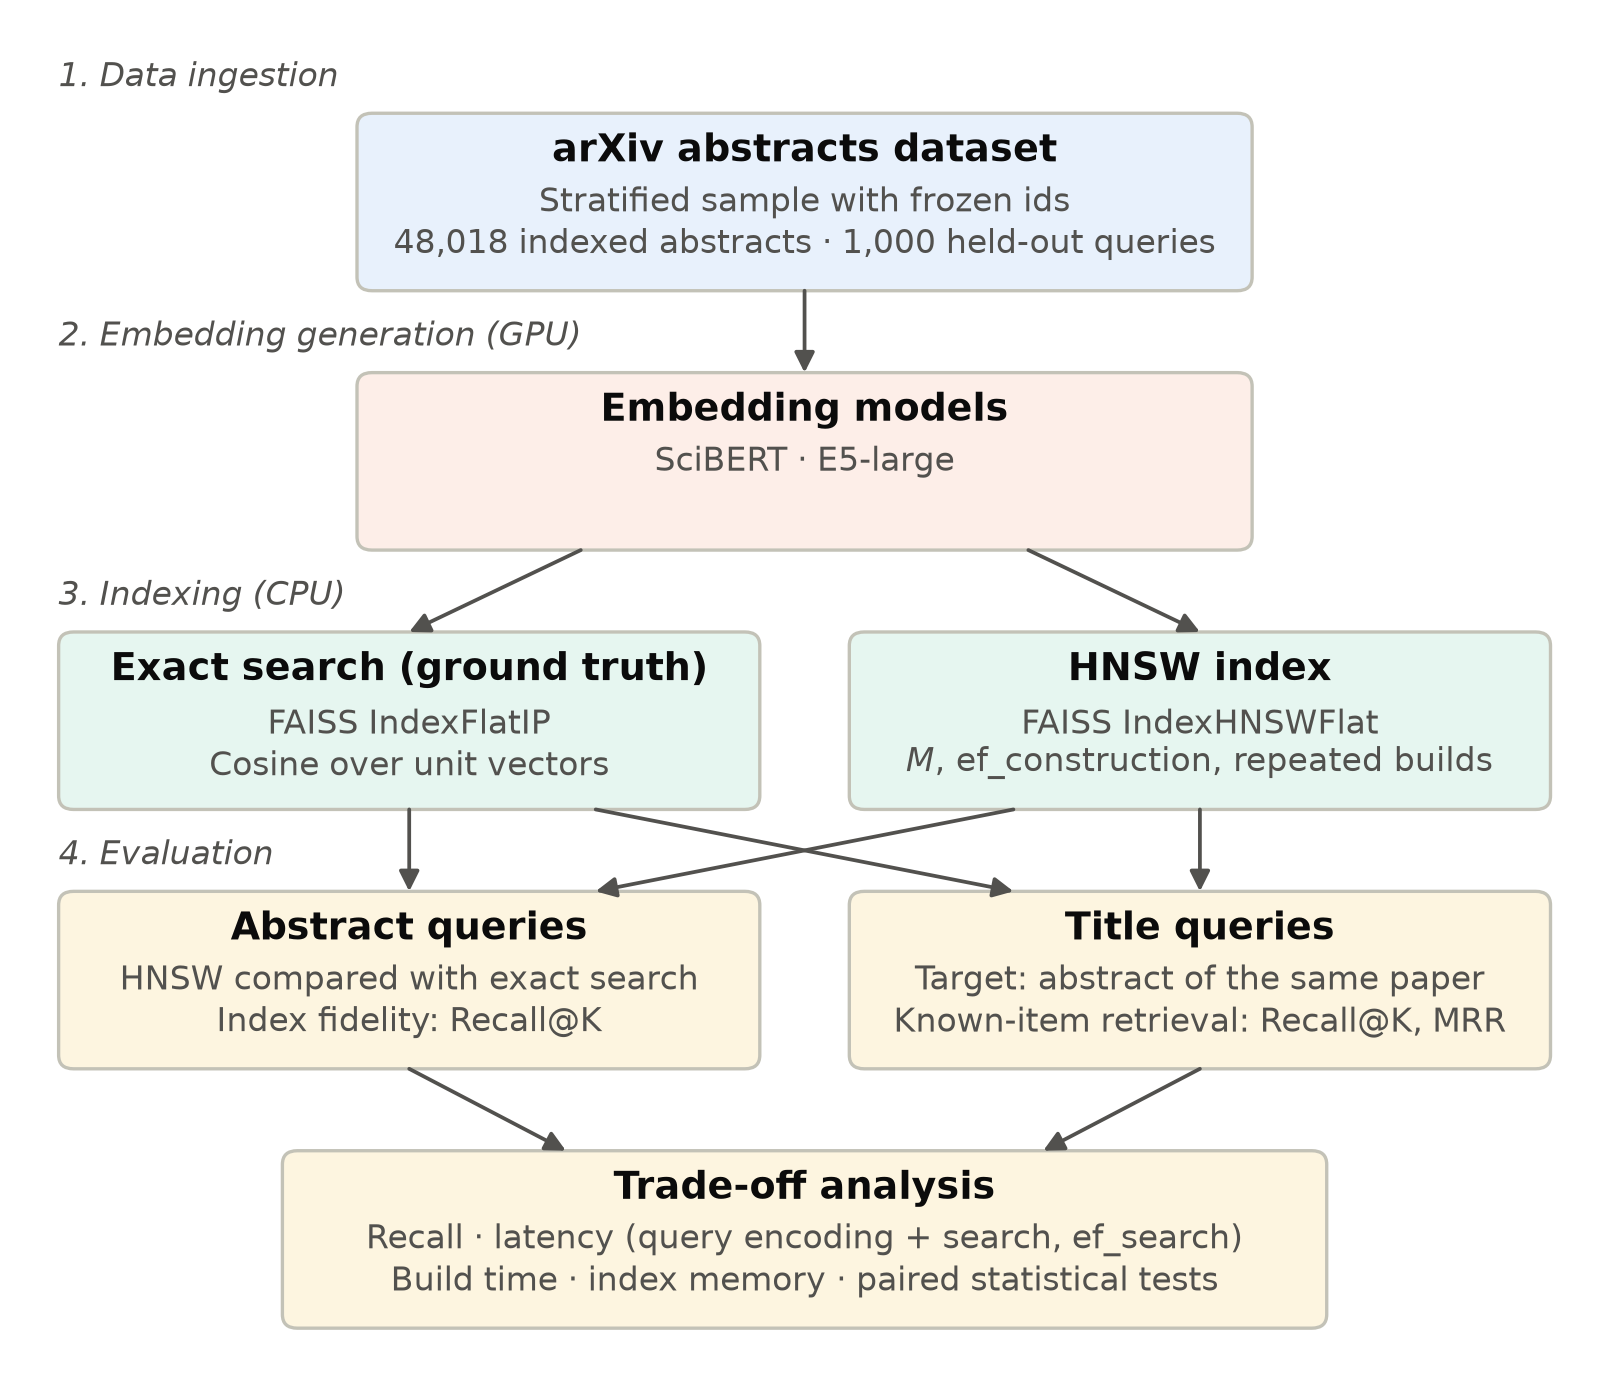
\includegraphics[width=0.86\columnwidth]{diagrama_bloques.png}
\caption{Experimental pipeline. Abstract queries measure the fidelity of HNSW to exact search; title queries measure retrieval of the abstract of the same paper.}
\label{fig:pipeline}
\end{figure}

\subsection{Dataset and Queries}

We use arXiv-abstracts-2021 (CC0 license), about two million arXiv abstracts \cite{clement2019}. A sample of 50,000 abstracts was drawn stratified by arXiv category, so that large areas such as physics do not crowd out small ones, and 1,000 of them were drawn as queries. Each record keeps its identifier, title, abstract and categories. An error in the original split discarded 982 non-query abstracts and left 982 queries inside the index; we removed those queries instead of resampling, which leaves 48,018 indexed abstracts, disjoint from the 1,000 queries. Both identifier lists are frozen.

The query set is not proportional to the corpus. The strata were derived from a malformed category label that splits the sample into more than a thousand strata, most with a single document, and the sampler takes at least one document per stratum, so rare category combinations are over-represented among the queries. By top-level area, mathematics accounts for 20.2\,\% of the corpus but 9.4\,\% of the queries, computer science for 16.2\,\% and 6.3\,\%, and high-energy phenomenology for 6.0\,\% and 12.0\,\%. We report this composition rather than resample, because the title queries and all frozen results depend on these identifiers.

\subsection{Embedding Models}

The grid uses two contrasting models (Table~\ref{tab:modelspec}): SciBERT \cite{beltagy2019}, trained on scientific text but not for similarity, and E5-large \cite{wang2022}, a general-domain model trained on query--passage pairs. They differ in domain, training objective and size at once, so four more models are evaluated at the reference configuration to separate those factors: BERT \cite{devlin2019}, general and untrained for similarity; SciNCL \cite{ostendorff2022}, trained on citations starting from the weights of SciBERT; SPECTER2 \cite{singh2023}, also trained on citations, with a proximity adapter for documents and an ad-hoc query adapter for titles; and E5-base, a smaller version of E5-large. SciBERT versus BERT isolates the domain, SciBERT versus SciNCL the training objective, and E5-base versus E5-large the size.

SciNCL and SPECTER2 take the first token as the document vector, as their authors recommend; the other models average the token embeddings, and E5 prefixes documents with ``\texttt{passage: }'' and queries with ``\texttt{query: }''. Texts are truncated to 512 tokens and every vector is normalized to unit length. All models index the abstract alone: SciNCL and SPECTER2 are designed for ``title [SEP] abstract'', but indexing the title would place the answer of the title queries inside the index.

\begin{table}[!tb]
\centering
\begin{threeparttable}
\caption{Embedding Models, as Published on Hugging Face}
\label{tab:modelspec}
\footnotesize
\setlength{\tabcolsep}{4pt}
\begin{tabular}{@{}llcc@{}}
\toprule
\textbf{Model} & \textbf{Identifier} & \textbf{Pooling} & \textbf{Dim.} \\
\midrule
SciBERT  & {\scriptsize\texttt{allenai/scibert\_scivocab\_uncased}} & mean & 768 \\
E5-large & {\scriptsize\texttt{intfloat/e5-large-v2}} & mean$^{\mathrm{a}}$ & 1024 \\
BERT     & {\scriptsize\texttt{bert-base-uncased}} & mean & 768 \\
SciNCL   & {\scriptsize\texttt{malteos/scincl}} & first & 768 \\
SPECTER2 & {\scriptsize\texttt{allenai/specter2\_base}}$^{\mathrm{b}}$ & first & 768 \\
E5-base  & {\scriptsize\texttt{intfloat/e5-base-v2}} & mean$^{\mathrm{a}}$ & 768 \\
\bottomrule
\end{tabular}
\begin{tablenotes}
\scriptsize
\item SciBERT and E5-large are evaluated over the whole grid; the other models at the reference configuration. $^{\mathrm{a}}$With ``query:''/``passage:'' prefixes. $^{\mathrm{b}}$With the proximity and ad-hoc query adapters.
\end{tablenotes}
\end{threeparttable}
\end{table}

\subsection{Index Parameters and Experimental Grid}

We use FAISS \cite{johnson2021} (\texttt{IndexHNSWFlat}), which gives direct access to the graph parameters. Table~\ref{tab:params} summarizes the three parameters, the phase in which each acts and the effect we measured. The grid covers $M \in \{8,16,32\}$ and \efc{} $\in \{100,200,400\}$ for SciBERT and E5-large, which gives 18 indexes; each index is queried with \efs{} $\in \{10,20,50,100,200,400\}$, which gives 108 operating points.

Similarity is the cosine, computed as the inner product of unit vectors. The $L_2$ distance is not evaluated separately because, for unit vectors $\mathbf{a}$ and $\mathbf{b}$,
\begin{equation}
\lVert \mathbf{a}-\mathbf{b} \rVert^2 = 2 - 2\,\mathbf{a}\cdot\mathbf{b},
\label{eq:l2}
\end{equation}
so both metrics produce the same ranking and any difference between them would be construction noise.

\begin{table}[!tb]
\centering
\caption{Index Parameters, Phase, Role and Measured Effect}
\label{tab:params}
\footnotesize
\setlength{\tabcolsep}{3pt}
\begin{tabular}{@{}l l >{\raggedright\arraybackslash}p{2.55cm} >{\raggedright\arraybackslash}p{2.75cm}@{}}
\toprule
\textbf{Param.} & \textbf{Phase} & \textbf{Role} & \textbf{Measured effect} \\
\midrule
$M$ & Build & Links per node in each layer; sets the density of the graph & Largest effect on recall; memory grows only 4.6--6.1\,\% from 8 to 32 \\
\addlinespace
\textit{ef\_c} & Build & Candidate list used to choose the links of a new node & Build time $\times$2.9--3.3 from 100 to 400; mean Recall@10 $+$0.003 to $+$0.005 \\
\addlinespace
\textit{ef\_s} & Query & Candidate list explored per query; changes without rebuilding & Sets the recall--latency trade-off; the value needed for a target grows with $N$ \\
\bottomrule
\end{tabular}
\end{table}

\subsection{Index Fidelity and Known-Item Retrieval}

\textit{Index fidelity.} For each model, an exact index (\texttt{IndexFlatIP}) returns the true 10 nearest neighbors of every query abstract among the 48,018 indexed abstracts. The fidelity of HNSW is its Recall@$K$ for $K \in \{1,5,10\}$,
\begin{equation}
\mathrm{Recall@}K = \frac{1}{|Q|}\sum_{q \in Q} \frac{|H_K(q) \cap E_K(q)|}{K},
\label{eq:recall}
\end{equation}
where $Q$ is the set of queries and $H_K(q)$ and $E_K(q)$ are the first $K$ results of HNSW and of exact search for query $q$. This ground truth comes from the same vector space, not from human judgments, so it measures how faithful the index is to the model, not whether the results are relevant. MRR is not reported for fidelity: if HNSW finds the true nearest neighbor it ranks it first, so MRR equals Recall@1 in all 108 operating points.

\textit{Known-item retrieval.} Abstracts as queries do not reflect use, where a user types a short phrase. For 1,000 indexed documents, drawn with a fixed seed, the title is the query and the abstract of the same paper is the single relevant document; titles are never indexed. Recall@$K$ is then the fraction of titles whose abstract appears among the first $K$ results, and
\begin{equation}
\mathrm{MRR@}10 = \frac{1}{|Q|}\sum_{q \in Q} \frac{1}{\mathrm{rank}_q},
\label{eq:mrr}
\end{equation}
with $1/\mathrm{rank}_q = 0$ when the abstract is not among the first 10 \cite{manning2008}. Both are computed with exact search, which isolates the model, and with HNSW at the reference configuration, which adds the error of the index. This task is a proxy for relevance, not a substitute for human judgments.

\subsection{Measurement Protocol and Configuration Selection}

Each configuration is built five times, inserting the vectors in a different random order each time, so that differences between configurations can be compared with the variation between builds. Recall is reported as mean $\pm$ standard deviation over the builds, and times as the median, which resists interference from other processes. Search latency is measured one query at a time on a single thread, as a user would experience it, after 50 warm-up queries, and reported as mean and 95th percentile. Builds use 6 threads, and memory is the size of the serialized index.

Embeddings were computed on an NVIDIA T4 GPU in Google Colab. Everything else ran on an Intel Core i5-11400H (6 cores, 12 threads) with 16\,GB of RAM under Windows 11, with Python 3.11.9, FAISS 1.14.2, NumPy 2.4.4, SciPy 1.17.1, scikit-learn 1.9.0, PyTorch 2.12.0 (CPU), Transformers 5.10.2 and Sentence-Transformers 5.5.1. All experiments were run in one sequence with the computer otherwise idle.

No configuration is best on every cost, so we report the Pareto front over Recall@10, latency, build time and memory, and fix a single rule for the reference configuration: among the operating points that reach Recall@10 $\geq 0.99$ in both SciBERT and E5-large, the one with the lowest sum of their latencies. The target of 0.99 is a conventional value fixed before running the full grid, and all later experiments use this configuration.

\subsection{Statistical Tests}

Models are compared in pairs on the same queries, so the tests are paired and the unit is the query. Six pairs are tested: SciBERT against E5-large, SciNCL and SPECTER2; BERT against SciBERT; SciNCL against E5-base; and E5-base against E5-large. For fidelity, the Recall@10 of each query is averaged over the five builds and compared with the Wilcoxon signed-rank test \cite{wilcoxon1945}, discarding queries with no difference; the binary outcome ``all 10 true neighbors found'' is compared with the exact McNemar test \cite{mcnemar1947} in each build, keeping the largest $p$-value. For known-item retrieval, McNemar compares whether the relevant abstract is among the first 10 results, and Wilcoxon compares the reciprocal rank. We report the rank-biserial correlation $r$, computed with mid-ranks for ties, the 95\,\% confidence interval of the mean difference from 10,000 paired bootstrap resamples, and $p$-values adjusted with Holm's method \cite{holm1979} over the 24 tests, with $\alpha=0.05$. A non-significant result is read as ``no difference detected'', not as equivalence.

\subsection{Additional Experiments}

\textit{End-to-end latency.} For each model, 200 titles and 200 abstracts are encoded one at a time on the CPU with 6 threads and then searched with HNSW on one thread.

\textit{Index families.} With the same queries and ground truth we compare exact search; HNSW at the reference $M$ and \efc{}; IVF-Flat, an inverted file with $4\sqrt{N}=876$ lists; IVF-PQ, the same with OPQ and product quantization into $d/16$ codes of 8 bits \cite{jegou2011,ge2014}, using $L_2$ on unit vectors; IVF-PQ with re-ranking of $10K$ candidates using the original vectors (IVF-PQ+Refine); and an exact ball tree from scikit-learn \cite{omohundro1989}. The inverted-file indexes sweep the number of lists visited from 1 to 256. Each family is built once.

\textit{Scalability.} Two larger pools are drawn from the dataset: 100,000 abstracts encoded with SciBERT, from which the 303 queries they contain are removed, and 500,000 abstracts encoded with E5-base, sampled after excluding the queries. Nested subsets from 5,000 vectors up to the whole pool are indexed with the reference $M$ and \efc{}, three builds per size (one at 500,000). The exact ground truth is recomputed at each size, and \efs{} is swept from 10 to 800 so that HNSW is compared with exact search at constant recall rather than at a fixed \efs{}. We fit the slope of $\log(\text{latency})$ against $\log N$ with its 95\,\% confidence interval, and time exact search on 200 queries. Batch latency, with all queries submitted together on 12 threads, is reported separately because it is the setting in which exact search benefits from optimized matrix products.

\textit{Implementation.} The pipeline is written in Python; every path, parameter and random seed lives in one configuration file, and every table in Section~\ref{sec:results} is generated from the result files. A Streamlit demonstration encodes a user query with E5-large, searches the HNSW index at the reference configuration and reports encoding and search times separately. Code and data availability are given at the end of the paper.

% =====================================================================
\section{Results}
\label{sec:results}
% =====================================================================

\subsection{Index Fidelity over the Parameter Grid}

Table~\ref{tab:configs} lists the 18 indexes at \efs{}$\,=100$ and Fig.~\ref{fig:latency} shows all 108 operating points. $M$ has the largest effect. At \efc{}$\,=100$, raising $M$ from 8 to 16 lifts Recall@10 from 0.967 to 0.993 with SciBERT and from 0.943 to 0.983 with E5-large; from 16 to 32 the gain shrinks to 0.005 and 0.009. Memory barely depends on $M$: from 8 to 32 the index grows by 6.1\,\% with SciBERT and 4.6\,\% with E5-large, because the vectors themselves dominate.

\efc{} is much less useful. Raising it from 100 to 400 multiplies build time by 2.9--3.3, for a mean gain in Recall@10, over all $M$ and \efs{}, of 0.005 with SciBERT and 0.003 with E5-large. When the index has to be rebuilt often, it is cheaper to keep \efc{} low and raise $M$ or \efs{} to reach the same recall. The variation between builds is small: the standard deviation of Recall@10 does not exceed 0.007 in any operating point.

\begin{table}[!tb]
\centering
\begin{threeparttable}
\caption{Fidelity and Cost of the 18 Indexes over Five Builds}
\label{tab:configs}
\footnotesize
\setlength{\tabcolsep}{3.2pt}
\begin{tabular}{@{}lcccccccc@{}}
\toprule
\textbf{Model} & $\boldsymbol{M}$ & \textbf{\textit{ef\_c}} & \textbf{R@1} & \textbf{R@5} & \textbf{R@10} & \textbf{ms} & \textbf{Build (s)} & \textbf{MB} \\
\midrule
\multirow{9}{*}{SciBERT}
 & 8 & 100 & 0.978 & 0.973 & 0.967$\pm$0.002 & 0.32 & 7.0 & 144 \\
 & 8 & 200 & 0.983 & 0.978 & 0.972$\pm$0.002 & 0.31 & 12.1 & 144 \\
 & 8 & 400 & 0.984 & 0.979 & 0.973$\pm$0.001 & 0.34 & 20.6 & 144 \\
 & 16 & 100 & 0.996 & 0.994 & 0.993$\pm$0.001 & 0.47 & 10.0 & 147 \\
 & 16 & 200 & 0.998 & 0.996 & 0.995$\pm$0.000 & 0.50 & 17.5 & 147 \\
 & 16 & 400 & 0.999 & 0.997 & 0.995$\pm$0.001 & 0.54 & 29.5 & 147 \\
 & 32 & 100 & 0.999 & 0.998 & 0.997$\pm$0.000 & 0.60 & 12.0 & 153 \\
 & 32 & 200 & 1.000 & 0.999 & 0.998$\pm$0.000 & 0.66 & 21.1 & 153 \\
 & 32 & 400 & 1.000 & 0.999 & 0.998$\pm$0.000 & 0.71 & 35.4 & 153 \\
\midrule
\multirow{9}{*}{E5-large}
 & 8 & 100 & 0.970 & 0.959 & 0.943$\pm$0.001 & 0.42 & 9.8 & 191 \\
 & 8 & 200 & 0.974 & 0.963 & 0.947$\pm$0.001 & 0.42 & 16.8 & 191 \\
 & 8 & 400 & 0.975 & 0.964 & 0.949$\pm$0.002 & 0.39 & 28.3 & 191 \\
 & 16 & 100 & 0.993 & 0.989 & 0.983$\pm$0.000 & 0.66 & 15.6 & 194 \\
 & 16 & 200 & 0.995 & 0.991 & 0.985$\pm$0.001 & 0.67 & 28.3 & 194 \\
 & 16 & 400 & 0.994 & 0.991 & 0.985$\pm$0.001 & 0.65 & 48.5 & 194 \\
 & 32 & 100 & 0.998 & 0.995 & 0.992$\pm$0.001 & 0.87 & 19.7 & 200 \\
 & 32 & 200 & 0.999 & 0.997 & 0.994$\pm$0.001 & 0.98 & 37.0 & 200 \\
 & 32 & 400 & 1.000 & 0.997 & 0.995$\pm$0.001 & 1.09 & 64.2 & 200 \\
\bottomrule
\end{tabular}
\begin{tablenotes}
\scriptsize
\item All indexes queried with \textit{ef\_search}\,=\,100. Recall: mean ($\pm$ s.d. for R@10); times: median. ms: search latency per query on one thread.
\end{tablenotes}
\end{threeparttable}
\end{table}

\begin{figure}[!tb]
\centering
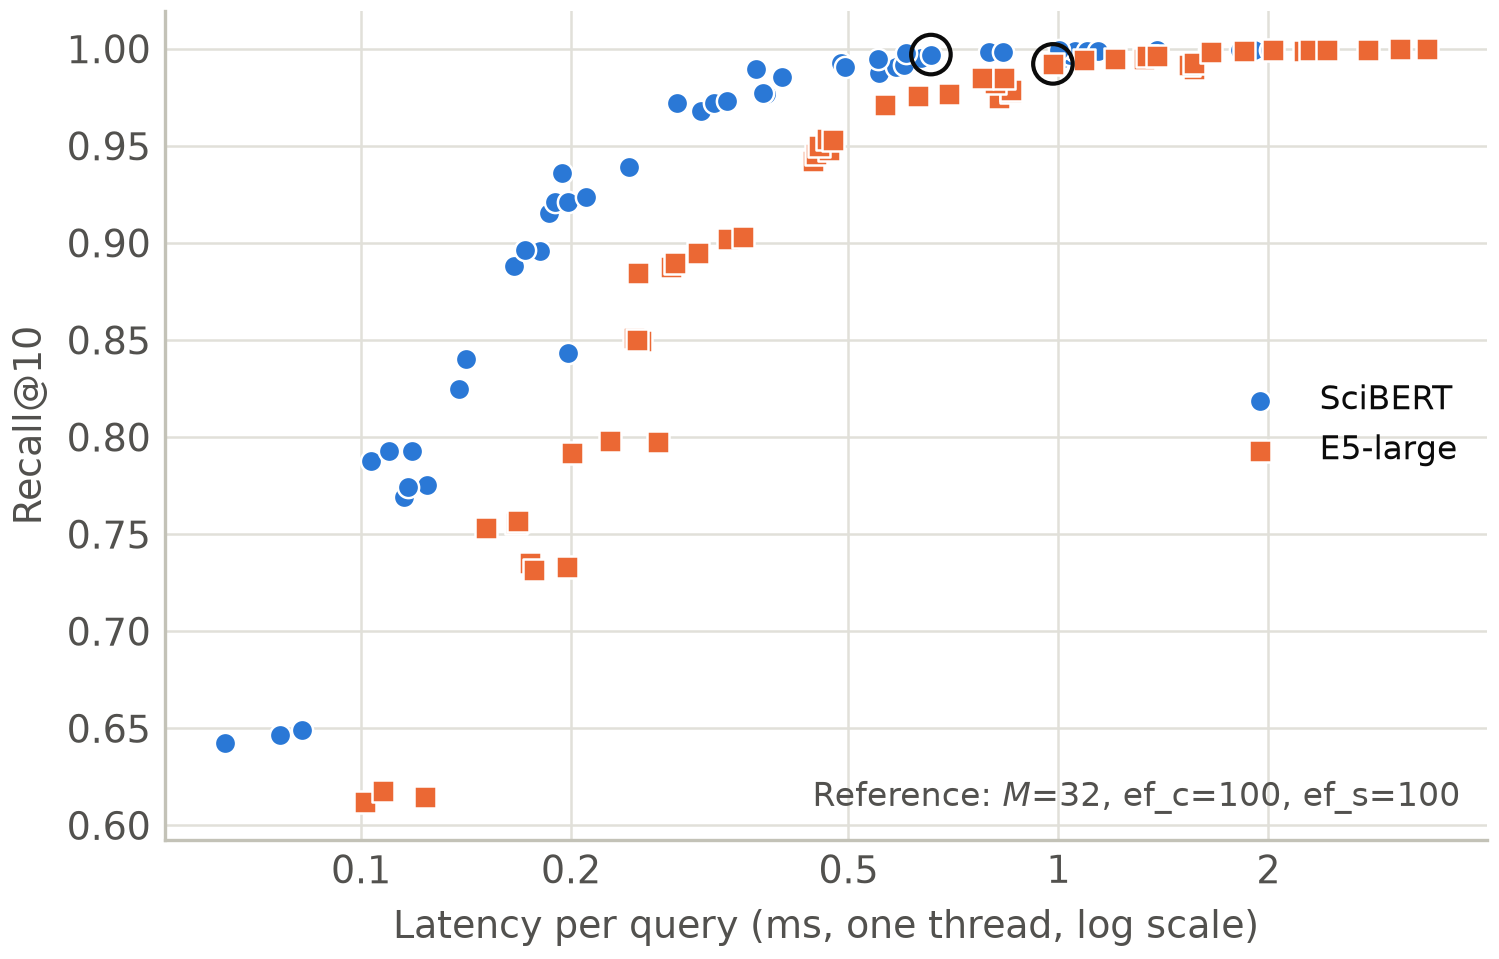
\includegraphics[width=\columnwidth]{fig_recall_latency.png}
\caption{Recall@10 against latency per query (one thread) for the 108 operating points; 48 of them lie on the Pareto front over recall, latency, build time and memory. Circles: reference configuration.}
\label{fig:latency}
\end{figure}

\subsection{Query-Time Search Breadth and the Reference Configuration}

\efs{} controls the trade-off at query time (Fig.~\ref{fig:efsearch}). With $M=32$ and \efc{}$\,=100$, Recall@10 rises from 0.825 at \efs{}$\,=10$ to 0.997 at 100 with SciBERT, and from 0.792 to 0.992 with E5-large; latency grows more slowly than \efs{}, which multiplied by 40 multiplies latency by 12 to 13. A common default of \efs{}$\,=50$ is not enough for E5-large, which stays at 0.971, and with it the lowest Recall@10 over the 18 indexes is 0.883 (E5-large, $M=8$, \efc{}$\,=100$).

The selection rule gives $M=32$, \efc{}$\,=100$ and \efs{}$\,=100$, with Recall@10 of $0.997 \pm 0.000$ and $0.992 \pm 0.001$, 0.60 and 0.87\,ms per query, 12 and 20\,s of build time, and 153 and 200\,MB, for SciBERT and E5-large. Other costs or targets lead to other choices. At the 0.95 target, $M=16$ with \efs{}$\,=50$ is the fastest point for both models (0.28 and 0.37\,ms). At the 0.99 target, the cheapest index to build uses $M=8$ with \efs{}$\,=400$ for SciBERT (7.0\,s, 1.07\,ms) and $M=16$ with \efs{}$\,=200$ for E5-large (15.6\,s, 1.13\,ms), and the smallest index uses $M=8$ for both models.

\begin{figure}[!tb]
\centering
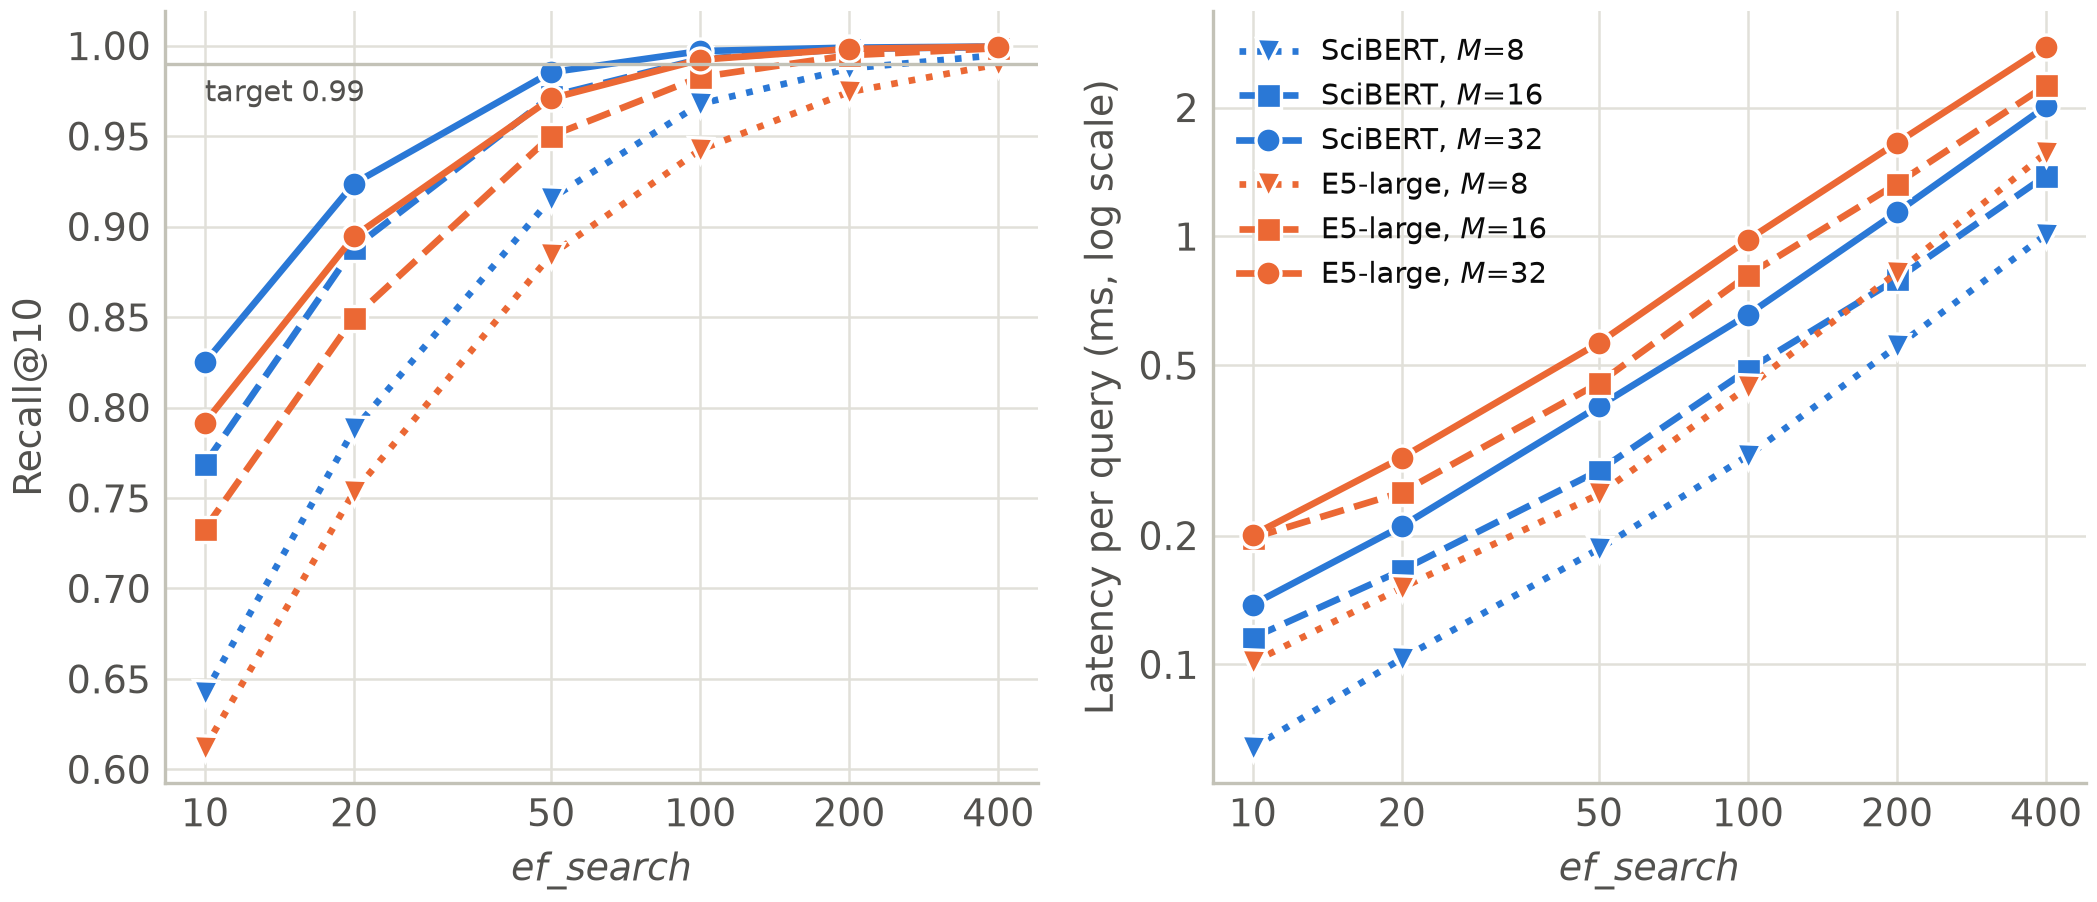
\includegraphics[width=\columnwidth]{fig_ef_search.png}
\caption{Recall@10 (left) and latency per query (right) against \textit{ef\_search} for each $M$, with \textit{ef\_construction}\,=\,100; mean and median over five builds.}
\label{fig:efsearch}
\end{figure}

\subsection{Index Fidelity versus Retrieval Quality}

The two evaluations rank the models in opposite orders (Table~\ref{tab:models}, Fig.~\ref{fig:natural}). In fidelity, SciBERT is ahead of E5-large by 0.005 in Recall@10 (95\,\% CI from $+0.0035$ to $+0.0071$, $p_{\mathrm{Holm}} = 1.4 \times 10^{-8}$), a small difference but larger than the variation between builds. When titles are the queries, E5-large finds the abstract of the same paper among the first 10 results for 949 of 1,000 titles and SciBERT for 173, with exact search; in 777 cases only E5-large succeeds and in 1 case only SciBERT. The median rank of the relevant abstract is 1 for E5-large and 259 for SciBERT.

The similarities explain the gap. With SciBERT, a title is on average closer to other abstracts (0.790 to the top-ranked one) than to its own (0.731); with E5-large both values are close (0.877 and 0.875), and the closest abstract is usually the right one. HNSW adds little error to this task: replacing exact search with the index lowers Recall@10 by 0.005 to 0.031 depending on the model.

\begin{table*}[!t]
\centering
\begin{threeparttable}
\caption{Index Fidelity and Known-Item Retrieval of the Six Models at the Reference Configuration}
\label{tab:models}
\footnotesize
\setlength{\tabcolsep}{4.2pt}
\begin{tabular}{@{}lllc cc ccccc c cc@{}}
\toprule
 & & & & \multicolumn{2}{c}{\textbf{Fidelity}} & \multicolumn{5}{c}{\textbf{Title$\rightarrow$abstract, exact search}} & \textbf{HNSW} & \multicolumn{2}{c}{\textbf{Similarity}} \\
\cmidrule(lr){5-6}\cmidrule(lr){7-11}\cmidrule(lr){12-12}\cmidrule(l){13-14}
\textbf{Model} & \textbf{Domain} & \textbf{Training} & \textbf{Dim.} & \textbf{R@10} & \textbf{ms} & \textbf{R@1} & \textbf{R@5} & \textbf{R@10} & \textbf{MRR@10} & \textbf{Med. rank} & \textbf{R@10} & \textbf{Own} & \textbf{Top-1} \\
\midrule
SciBERT  & Scientific & None           & 768  & 0.997 & 0.60 & 0.061 & 0.131 & 0.173 & 0.093 & 259 & 0.164 & 0.731 & 0.790 \\
SciNCL   & Scientific & Citations      & 768  & 0.998 & 0.45 & 0.527 & 0.700 & 0.746 & 0.600 & 1   & 0.733 & 0.909 & 0.922 \\
SPECTER2 & Scientific & Citations      & 768  & 0.998 & 0.63 & 0.539 & 0.698 & 0.754 & 0.607 & 1   & 0.723 & 0.774 & 0.784 \\
BERT     & General    & None           & 768  & 0.996 & 0.58 & 0.064 & 0.132 & 0.175 & 0.094 & 280 & 0.160 & 0.771 & 0.835 \\
E5-base  & General    & Query--passage & 768  & 0.986 & 0.75 & 0.813 & 0.900 & 0.922 & 0.851 & 1   & 0.913 & 0.875 & 0.879 \\
E5-large & General    & Query--passage & 1024 & 0.992 & 0.87 & 0.869 & 0.941 & 0.949 & 0.899 & 1   & 0.944 & 0.875 & 0.877 \\
\bottomrule
\end{tabular}
\begin{tablenotes}
\scriptsize
\item Reference configuration: $M=32$, \textit{ef\_construction}\,=\,100, \textit{ef\_search}\,=\,100. Fidelity: abstract$\rightarrow$abstract Recall@10 of HNSW against exact search, and search latency on one thread. Title$\rightarrow$abstract: 1,000 titles, each with its own abstract as the single relevant document. Similarity: mean cosine between a title and its own abstract, and between a title and the top-ranked document.
\end{tablenotes}
\end{threeparttable}
\end{table*}

\begin{figure}[!tb]
\centering
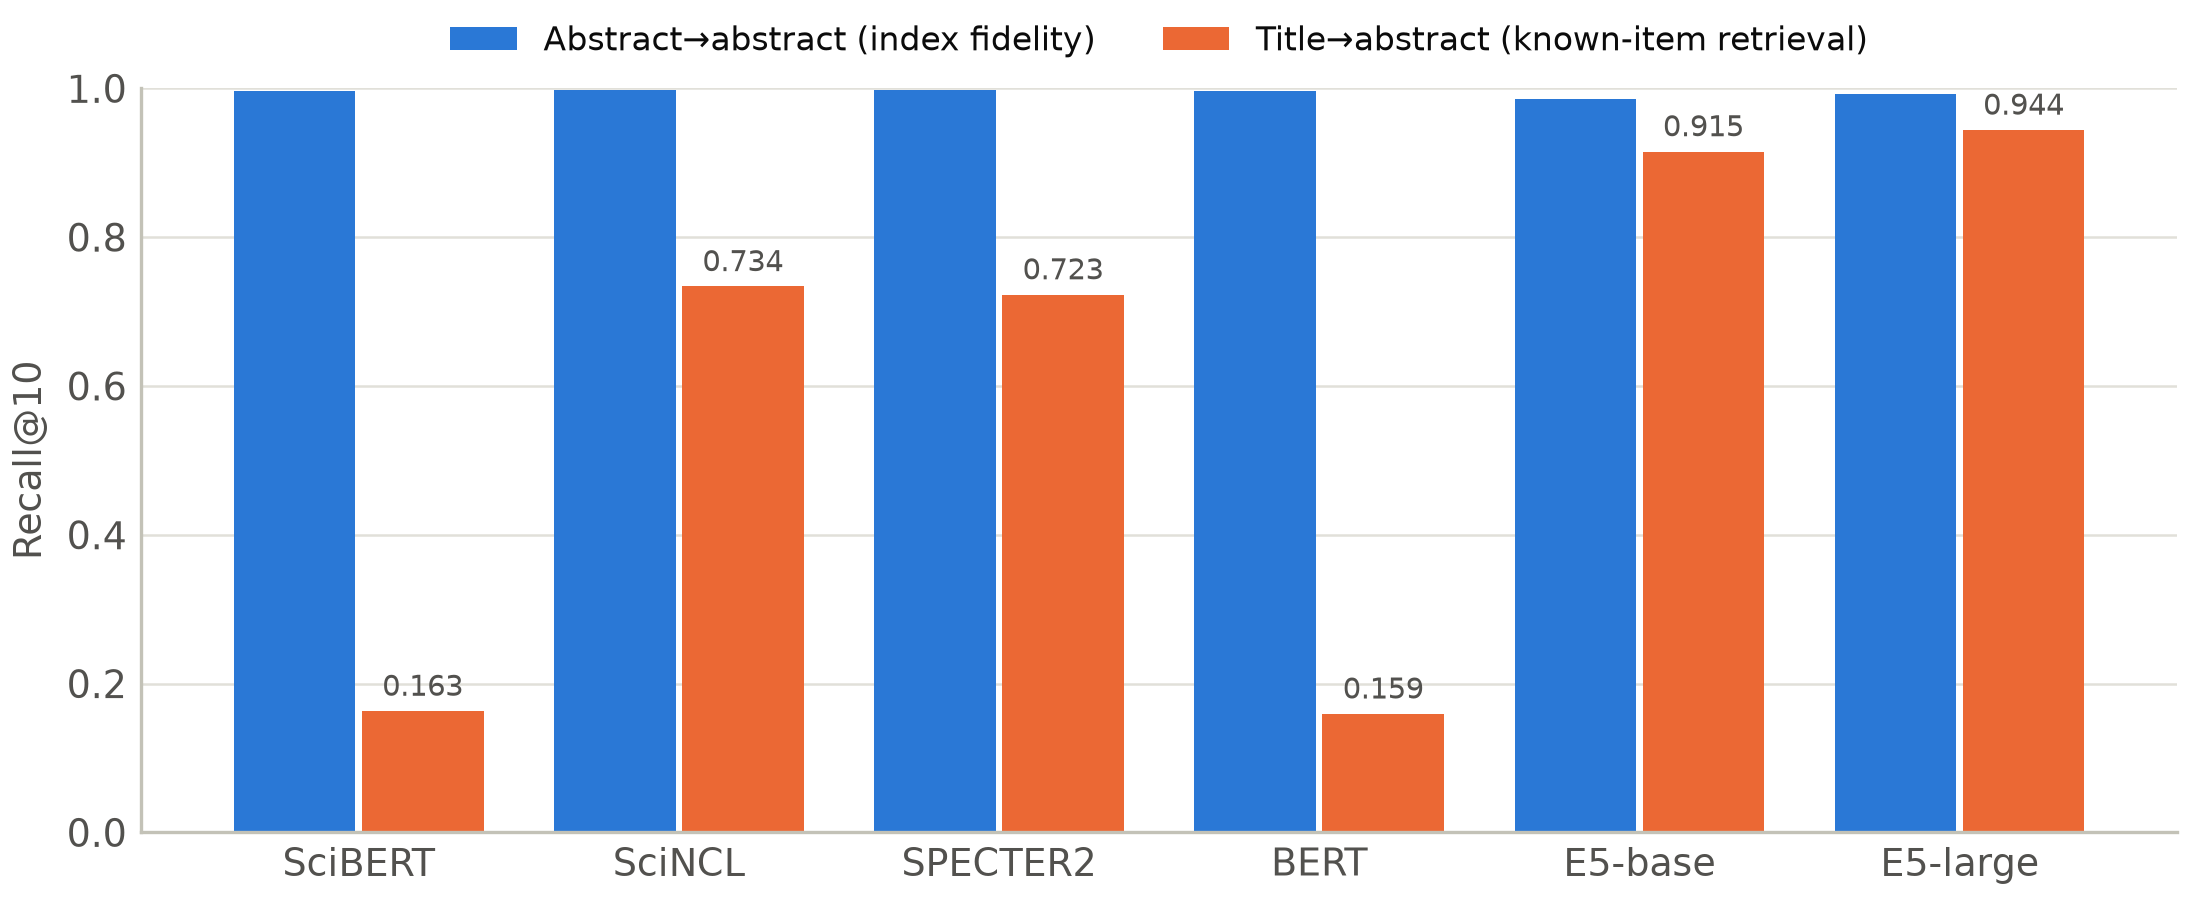
\includegraphics[width=\columnwidth]{fig_natural_vs_fidelity.png}
\caption{Recall@10 of the six models at the reference configuration. Abstract$\rightarrow$abstract: fidelity of HNSW to exact search. Title$\rightarrow$abstract: retrieval of the abstract of the same paper with HNSW.}
\label{fig:natural}
\end{figure}

\subsection{Domain versus Training Objective}

Table~\ref{tab:models} crosses domain and training objective, and Table~\ref{tab:significance} lists every test. The scientific domain alone makes no detectable difference: BERT and SciBERT reach 0.175 and 0.173 in title$\rightarrow$abstract Recall@10 ($p_{\mathrm{Holm}}=1.00$). The training objective does: SciNCL, which starts from the weights of SciBERT and is trained on citations, reaches 0.746, and SPECTER2 reaches 0.754 ($p_{\mathrm{Holm}}<10^{-10}$ against SciBERT in both cases). Among models trained for similarity, E5-base reaches 0.922 against 0.746 for SciNCL at the same dimension; this contrast changes the domain and the kind of training at once, so it cannot be attributed to either one. Size helps within a family: E5-large improves on E5-base by 0.027 ($p_{\mathrm{Holm}}=4.6 \times 10^{-4}$).

Fidelity, in contrast, hardly depends on the model: all six lie between 0.986 and 0.998. Nor is it explained by dimension: E5-base has fewer dimensions than E5-large and lower fidelity, and among the 768-dimensional models the search takes from 0.45 to 0.75\,ms.

\begin{table*}[!t]
\centering
\begin{threeparttable}
\caption{Paired Tests at the Reference Configuration, Holm-Adjusted over 24 Tests}
\label{tab:significance}
\footnotesize
\setlength{\tabcolsep}{4.5pt}
\begin{tabular}{@{}l ccc c c cc c@{}}
\toprule
 & \multicolumn{5}{c}{\textbf{Wilcoxon signed-rank}} & \multicolumn{3}{c}{\textbf{Exact McNemar}} \\
\cmidrule(lr){2-6}\cmidrule(l){7-9}
\textbf{Pair (A vs B)} & \textbf{Means A / B} & $\boldsymbol{n}$ & $\boldsymbol{r}$ & \textbf{95\,\% CI of A$-$B} & $\boldsymbol{p_{\mathrm{Holm}}}$ & \textbf{Means A / B} & $\boldsymbol{b}$\,;\,$\boldsymbol{c}$ & $\boldsymbol{p_{\mathrm{Holm}}}$ \\
\midrule
\multicolumn{9}{@{}l}{\textit{Fidelity (abstract$\rightarrow$abstract): Wilcoxon on Recall@10; McNemar on ``all 10 true neighbors found''}} \\
SciBERT vs E5-large  & 0.997 / 0.992 & 225 & $+0.462$ & [$+0.0035$, $+0.0071$] & $1.4\times10^{-8}$ & 0.974 / 0.931 & 56--74\,;\,21--31 & $4.9\times10^{-3}$ \\
SciBERT vs SciNCL    & 0.997 / 0.998 & 107 & $-0.252$ & [$-0.0022$, $-0.0002$] & 0.16 & 0.974 / 0.984 & 11--19\,;\,21--30 & 1.00 \\
SciBERT vs SPECTER2  & 0.997 / 0.998 & 129 & $-0.171$ & [$-0.0019$, $+0.0002$] & 0.57 & 0.974 / 0.980 & 15--23\,;\,23--32 & 1.00 \\
BERT vs SciBERT      & 0.996 / 0.997 & 135 & $-0.097$ & [$-0.0019$, $+0.0004$] & 1.00 & 0.968 / 0.974 & 19--28\,;\,24--30 & 1.00 \\
SciNCL vs E5-base    & 0.998 / 0.986 & 274 & $+0.861$ & [$+0.0103$, $+0.0140$] & $<10^{-10}$ & 0.984 / 0.882 & 107--126\,;\,8--17 & $<10^{-10}$ \\
E5-base vs E5-large  & 0.986 / 0.992 & 323 & $-0.378$ & [$-0.0080$, $-0.0035$] & $3.6\times10^{-8}$ & 0.882 / 0.931 & 48--57\,;\,91--111 & $9.0\times10^{-3}$ \\
\midrule
\multicolumn{9}{@{}l}{\textit{Known-item retrieval (title$\rightarrow$abstract, exact search): Wilcoxon on reciprocal rank (RR@10); McNemar on hit@10}} \\
SciBERT vs E5-large  & 0.093 / 0.899 & 888 & $-0.997$ & [$-0.8279$, $-0.7848$] & $<10^{-10}$ & 0.173 / 0.949 & 1\,;\,777 & $<10^{-10}$ \\
SciBERT vs SciNCL    & 0.093 / 0.600 & 705 & $-0.958$ & [$-0.5362$, $-0.4785$] & $<10^{-10}$ & 0.173 / 0.746 & 12\,;\,585 & $<10^{-10}$ \\
SciBERT vs SPECTER2  & 0.093 / 0.607 & 719 & $-0.950$ & [$-0.5440$, $-0.4849$] & $<10^{-10}$ & 0.173 / 0.754 & 15\,;\,596 & $<10^{-10}$ \\
BERT vs SciBERT      & 0.094 / 0.093 & 224 & $+0.022$ & [$-0.0152$, $+0.0169$] & 1.00 & 0.175 / 0.173 & 79\,;\,77 & 1.00 \\
SciNCL vs E5-base    & 0.600 / 0.851 & 440 & $-0.842$ & [$-0.2776$, $-0.2237$] & $<10^{-10}$ & 0.746 / 0.922 & 21\,;\,197 & $<10^{-10}$ \\
E5-base vs E5-large  & 0.851 / 0.899 & 140 & $-0.706$ & [$-0.0612$, $-0.0360$] & $<10^{-10}$ & 0.922 / 0.949 & 8\,;\,35 & $4.6\times10^{-4}$ \\
\bottomrule
\end{tabular}
\begin{tablenotes}
\scriptsize
\item $n$: queries with a non-zero difference; $r$: rank-biserial correlation; CI: 95\,\% paired bootstrap interval of the mean difference; $b$, $c$: discordant queries (A only, B only). For fidelity, McNemar is run in each of the five builds and $b$, $c$ give the range over builds.
\end{tablenotes}
\end{threeparttable}
\end{table*}

\subsection{End-to-End Latency}

Searching the index is not the bottleneck (Table~\ref{tab:e2e}). Encoding a title on the CPU takes 37\,ms with SciBERT and 165\,ms with E5-large, and an abstract 149 and 562\,ms, while the search takes less than 1\,ms; encoding is 98.1--99.8\,\% of the total. E5-base encodes titles 3.5 times faster than E5-large (47 against 165\,ms) and loses 0.027 in title$\rightarrow$abstract Recall@10. The encoding time of SPECTER2 was not measured, because its adapter library requires a different version of Transformers.

\begin{table}[!tb]
\centering
\begin{threeparttable}
\caption{End-to-End Latency per Query on the CPU (ms)}
\label{tab:e2e}
\footnotesize
\setlength{\tabcolsep}{4pt}
\begin{tabular}{@{}l ccc ccc@{}}
\toprule
 & \multicolumn{3}{c}{\textbf{Title}} & \multicolumn{3}{c}{\textbf{Abstract}} \\
\cmidrule(lr){2-4}\cmidrule(l){5-7}
\textbf{Model} & \textbf{Encode} & \textbf{p95} & \textbf{Search} & \textbf{Encode} & \textbf{p95} & \textbf{Search} \\
\midrule
SciBERT  & 37  & 43  & 0.46 & 149 & 266 & 0.68 \\
E5-large & 165 & 189 & 0.85 & 562 & 993 & 0.94 \\
SciNCL   & 45  & 55  & 0.56 & 154 & 284 & 0.49 \\
BERT     & 46  & 53  & 0.41 & 165 & 301 & 0.49 \\
E5-base  & 47  & 57  & 0.91 & 159 & 279 & 0.87 \\
\bottomrule
\end{tabular}
\begin{tablenotes}
\scriptsize
\item 200 texts encoded one at a time with 6 threads, then searched with HNSW on one thread at the reference configuration. Encode: mean; p95: 95th percentile of encoding time. Encoding takes 98.1--99.8\,\% of the total.
\end{tablenotes}
\end{threeparttable}
\end{table}

\subsection{Other Index Families}

At the 0.99 target HNSW is the fastest family (Table~\ref{tab:families}, Fig.~\ref{fig:families}): 0.61\,ms with SciBERT and 0.73\,ms with E5-large, against 2.03 and 4.38\,ms for IVF-Flat. These values come from a single build of each family, so they differ slightly from the medians over five builds in Table~\ref{tab:configs} (0.60 and 0.87\,ms). IVF-Flat builds 4--6 times faster (2.7 and 3.3\,s against 11.9 and 19.2\,s) and is only about 1.5 times slower than HNSW at the 0.95 target with SciBERT. IVF-PQ with OPQ needs only 8 and 12\,MB, about 6\,\% of the exact index, but stops at a Recall@10 of 0.737 and 0.611. Re-ranking its candidates with the original vectors lets it reach the 0.99 target with SciBERT, at 1.21\,ms, but not with E5-large, where it stops at 0.983; it keeps the vectors, so it uses as much memory as HNSW, and building it, mostly training OPQ, takes 462 and 653\,s. The ball tree is exact but slower than exhaustive search (47 and 60\,ms against 10 and 12\,ms) and uses twice the memory: in 768 and 1,024 dimensions its partitions prune little.

\begin{table}[!tb]
\centering
\begin{threeparttable}
\caption{Index Families on the Same Queries and Ground Truth}
\label{tab:families}
\footnotesize
\setlength{\tabcolsep}{3.5pt}
\begin{tabular}{@{}lccccc@{}}
\toprule
 & \textbf{Best} & \multicolumn{2}{c}{\textbf{ms at R@10 $\geq$}} & \textbf{Build} & \\
\cmidrule(lr){3-4}
\textbf{Family} & \textbf{R@10} & \textbf{0.95} & \textbf{0.99} & \textbf{(s)} & \textbf{MB} \\
\midrule
\multicolumn{6}{@{}l}{\textit{SciBERT}} \\
Exact          & 0.999 & 10.19 & 10.19 & 0.0   & 141 \\
HNSW           & 1.000 & 0.38  & 0.61  & 11.9  & 153 \\
IVF-Flat       & 1.000 & 0.58  & 2.03  & 2.7   & 144 \\
IVF-PQ         & 0.737 & --    & --    & 461.6 & 8   \\
IVF-PQ+Refine  & 1.000 & 0.51  & 1.21  & 461.6 & 149 \\
Ball tree      & 0.999 & 46.85 & 46.85 & 5.7   & 294 \\
\midrule
\multicolumn{6}{@{}l}{\textit{E5-large}} \\
Exact          & 1.000 & 12.38 & 12.38 & 0.0   & 188 \\
HNSW           & 0.999 & 0.46  & 0.73  & 19.2  & 200 \\
IVF-Flat       & 0.998 & 1.32  & 4.38  & 3.3   & 191 \\
IVF-PQ         & 0.611 & --    & --    & 653.1 & 12  \\
IVF-PQ+Refine  & 0.983 & 1.79  & --    & 653.1 & 199 \\
Ball tree      & 1.000 & 59.64 & 59.64 & 9.3   & 392 \\
\bottomrule
\end{tabular}
\begin{tablenotes}
\scriptsize
\item One thread, one query at a time. Best R@10: highest Recall@10 over the search parameter; then the latency of the fastest setting reaching each target (--: not reached). Build time includes training.
\end{tablenotes}
\end{threeparttable}
\end{table}

\begin{figure*}[!t]
\centering
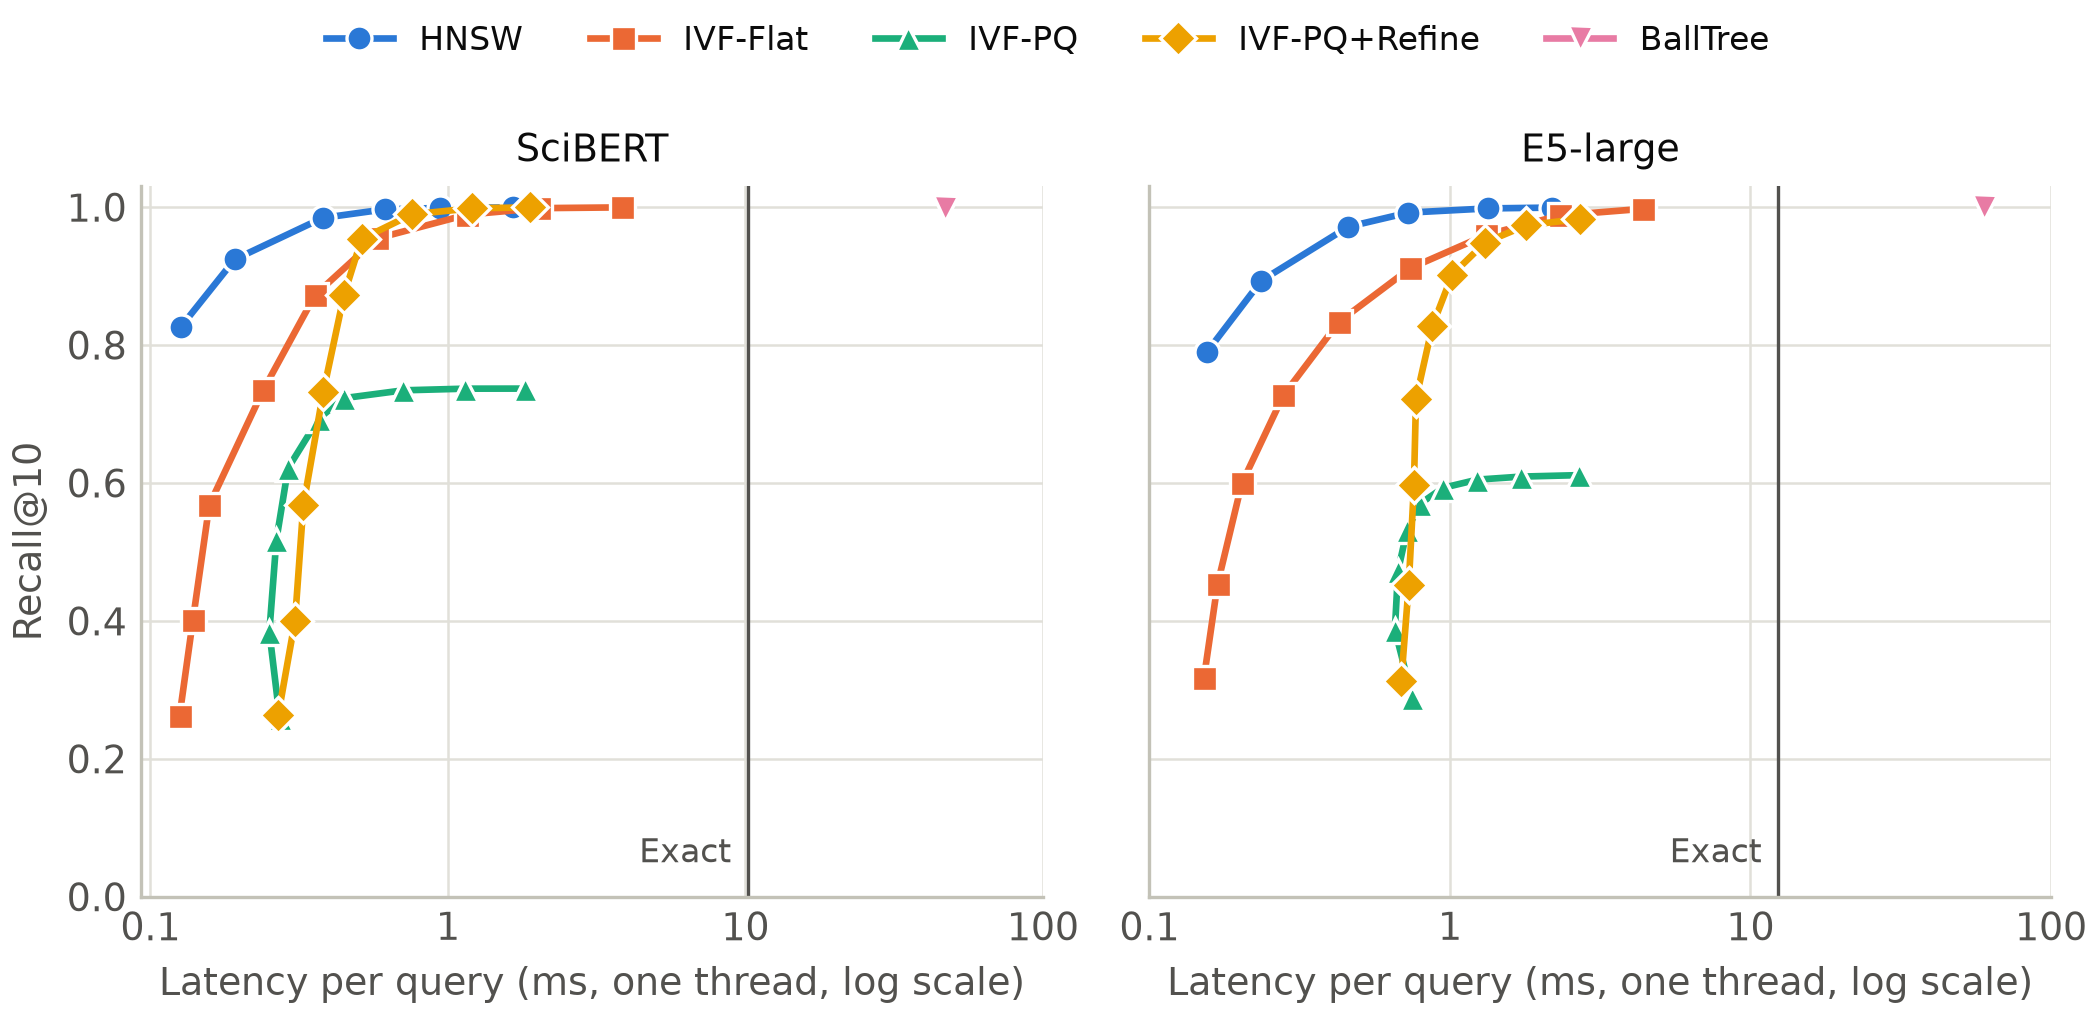
\includegraphics[width=0.64\textwidth]{fig_index_families.png}
\caption{Recall@10 against latency per query (one thread) for each index family, sweeping its search parameter. Vertical line: exhaustive search.}
\label{fig:families}
\end{figure*}

\subsection{Scalability}

At constant recall, HNSW is faster than exact search at every size measured, one query at a time (Table~\ref{tab:scalability}, Fig.~\ref{fig:scalability}). With E5-base, from 5,000 to 500,000 vectors, exact search goes from 1.1 to 107\,ms and HNSW at Recall@10 $\geq 0.99$ from 0.28 to 3.3\,ms, so the advantage grows from $4\times$ to $32\times$. The fitted slopes quantify the growth: 1.00 $[0.96, 1.04]$ for exact search, which is linear, and 0.53 $[0.48, 0.59]$ for HNSW at 0.99 (0.38 $[0.26, 0.51]$ at 0.95). With SciBERT up to 100,000 vectors the slopes are 1.00 $[0.92, 1.07]$ and 0.52 $[0.41, 0.63]$. HNSW is sublinear but not logarithmic in this range, partly because the \efs{} needed for a fixed recall grows with $N$, from 75 to 300 with E5-base. Building the 500,000-vector index takes 299\,s and 1.6\,GB.

The batch setting tells a different story. With all queries together on 12 threads, exact search uses optimized matrix products and is faster than HNSW at Recall@10 $\geq 0.99$ up to 200,000 vectors ($0.3\times$ to $0.6\times$); HNSW overtakes it only at 500,000 ($1.3\times$). At the 0.95 target, apart from the smallest size, the two are even at 100,000 and HNSW wins from 200,000. With SciBERT up to 100,000 vectors, the batch ratio at 0.99 stays between $0.7\times$ and $1.2\times$. The size at which HNSW pays off therefore depends on how queries are served, and not only on $N$.

\begin{table*}[!t]
\centering
\begin{threeparttable}
\caption{Latency against Corpus Size at Constant Recall}
\label{tab:scalability}
\footnotesize
\setlength{\tabcolsep}{5pt}
\begin{tabular}{@{}r c cccc cccc cc@{}}
\toprule
 & & \multicolumn{4}{c}{\textbf{R@10 $\geq$ 0.95}} & \multicolumn{4}{c}{\textbf{R@10 $\geq$ 0.99}} & & \\
\cmidrule(lr){3-6}\cmidrule(lr){7-10}
$\boldsymbol{N}$ & \textbf{Exact (ms)} & \textbf{\textit{ef\_s}} & \textbf{ms} & \textbf{Gain} & \textbf{Batch} & \textbf{\textit{ef\_s}} & \textbf{ms} & \textbf{Gain} & \textbf{Batch} & \textbf{Build (s)} & \textbf{MB} \\
\midrule
\multicolumn{12}{@{}l}{\textit{SciBERT}} \\
5,000   & 1.07  & 20 & 0.10 & 11$\times$ & 1.8$\times$ & 50  & 0.16 & 7$\times$  & 1.0$\times$ & 0  & 16  \\
10,000  & 2.13  & 20 & 0.12 & 18$\times$ & 1.4$\times$ & 50  & 0.21 & 10$\times$ & 0.7$\times$ & 1  & 32  \\
20,000  & 3.81  & 30 & 0.20 & 19$\times$ & 1.1$\times$ & 50  & 0.27 & 14$\times$ & 0.7$\times$ & 3  & 64  \\
50,000  & 10.74 & 30 & 0.27 & 40$\times$ & 1.7$\times$ & 75  & 0.50 & 22$\times$ & 0.9$\times$ & 12 & 159 \\
99,697  & 20.79 & 50 & 0.41 & 51$\times$ & 1.8$\times$ & 100 & 0.73 & 29$\times$ & 1.2$\times$ & 34 & 318 \\
\midrule
\multicolumn{12}{@{}l}{\textit{E5-base}} \\
5,000   & 1.10   & 30 & 0.16 & 7$\times$   & 1.1$\times$ & 75  & 0.28 & 4$\times$  & 0.6$\times$ & 0   & 16   \\
10,000  & 2.17   & 50 & 0.30 & 7$\times$   & 0.5$\times$ & 100 & 0.50 & 4$\times$  & 0.3$\times$ & 1   & 32   \\
20,000  & 3.83   & 50 & 0.34 & 11$\times$  & 0.5$\times$ & 100 & 0.63 & 6$\times$  & 0.3$\times$ & 4   & 64   \\
50,000  & 9.88   & 75 & 0.66 & 15$\times$  & 0.6$\times$ & 150 & 1.12 & 9$\times$  & 0.4$\times$ & 18  & 159  \\
100,000 & 21.18  & 75 & 0.74 & 29$\times$  & 1.0$\times$ & 200 & 1.51 & 14$\times$ & 0.5$\times$ & 45  & 319  \\
200,000 & 42.70  & 75 & 0.81 & 53$\times$  & 1.9$\times$ & 300 & 2.44 & 17$\times$ & 0.6$\times$ & 104 & 638  \\
500,000 & 106.88 & 75 & 1.00 & 107$\times$ & 4.8$\times$ & 300 & 3.34 & 32$\times$ & 1.3$\times$ & 299 & 1595 \\
\bottomrule
\end{tabular}
\begin{tablenotes}
\scriptsize
\item HNSW with $M=32$ and \textit{ef\_construction}\,=\,100. Exact and HNSW latency per query on one thread, one query at a time; HNSW uses the smallest \textit{ef\_search} reaching each Recall@10 target. Gain: speedup over exact search; Batch: the same ratio with all queries submitted together on 12 threads. Build time with 6 threads and size of the index.
\end{tablenotes}
\end{threeparttable}
\end{table*}

\begin{figure*}[!t]
\centering
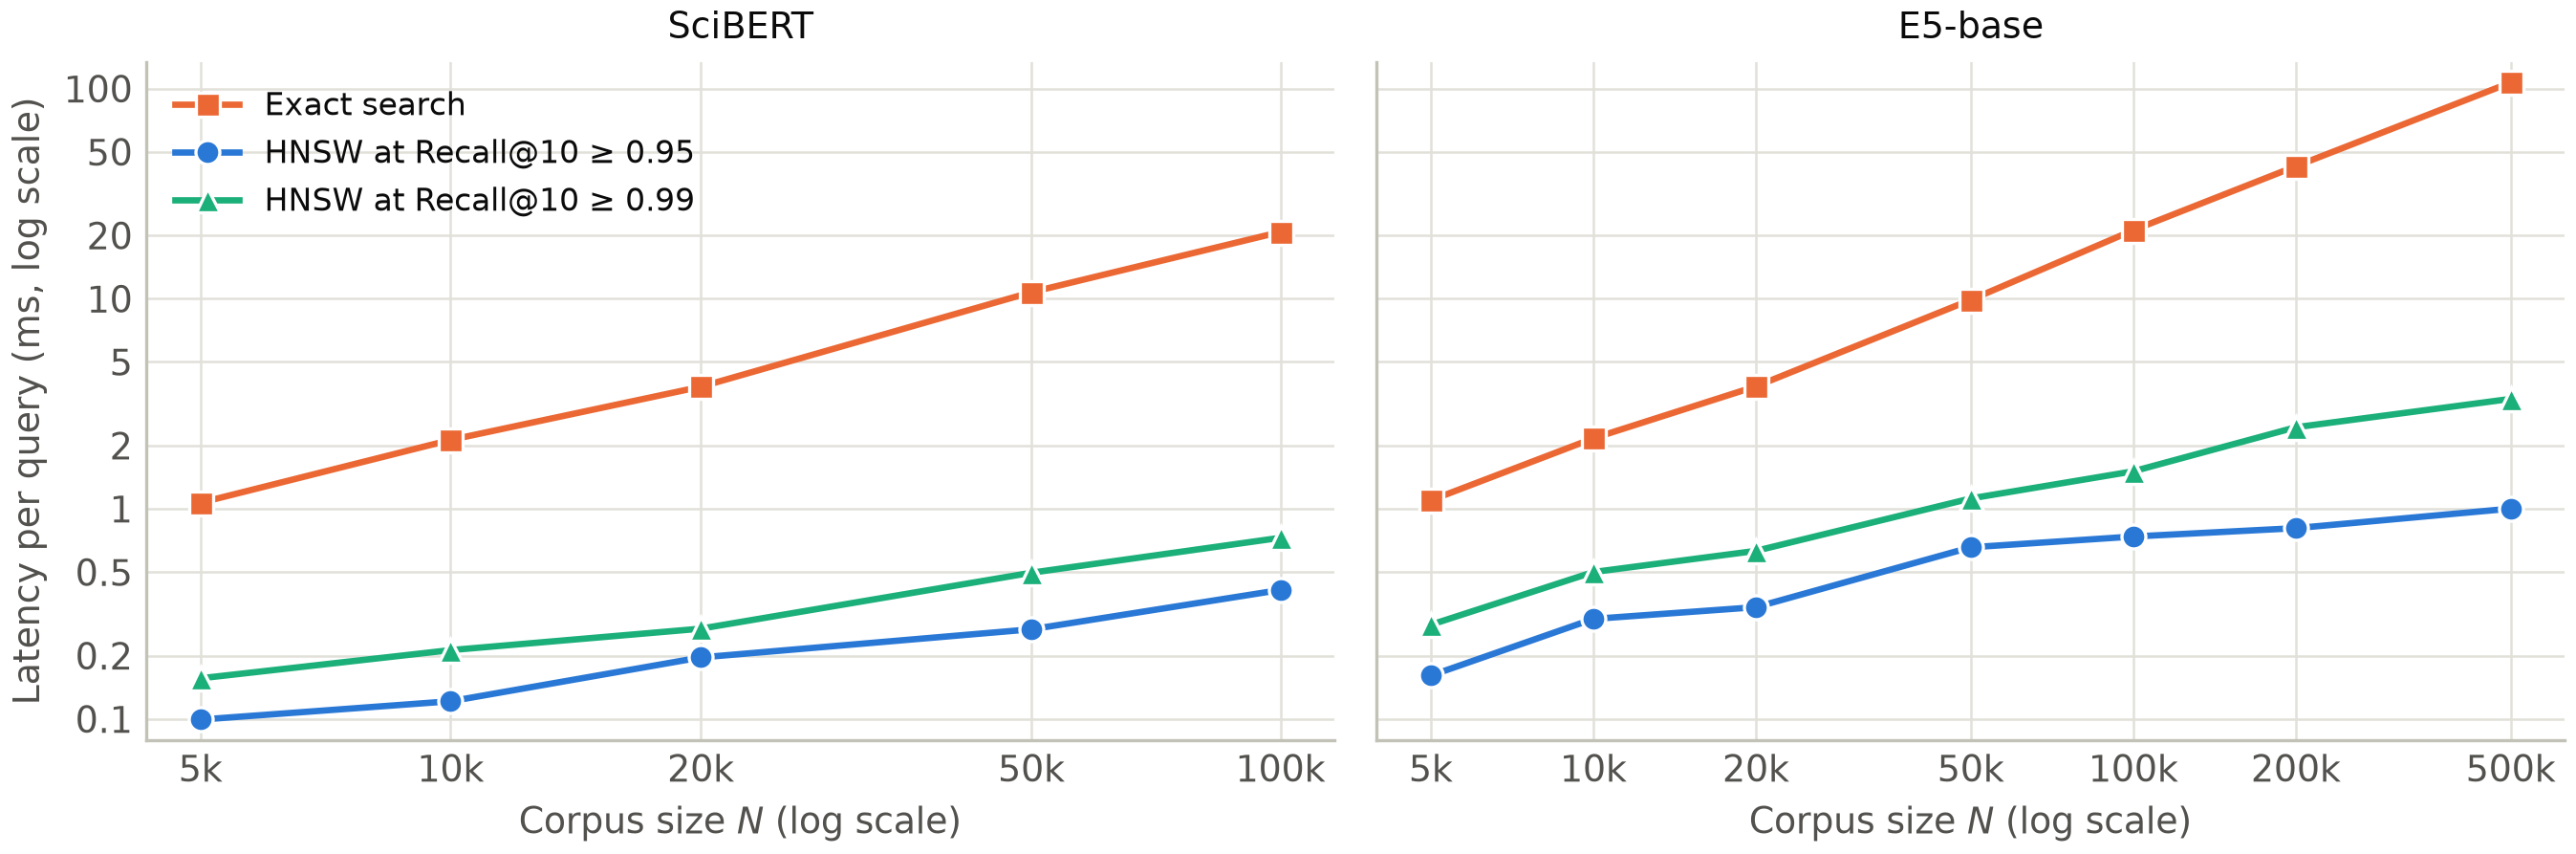
\includegraphics[width=0.76\textwidth]{fig_scalability.png}
\caption{Latency per query against corpus size, one thread and one query at a time, in log--log scale. HNSW uses the smallest \textit{ef\_search} reaching each Recall@10 target.}
\label{fig:scalability}
\end{figure*}

% =====================================================================
\section{Discussion}
\label{sec:discussion}
% =====================================================================

\subsection{Fidelity Is Not Relevance}

The central result is that index fidelity and retrieval quality are different dimensions. A Recall@10 of 0.997 says that HNSW reproduces exact search in the vector space of SciBERT; it says nothing about whether that space places a title near its own abstract. All six models keep a fidelity between 0.986 and 0.998, while their retrieval with exact search ranges from 0.17 to 0.95. Once $M$ and \efs{} are reasonable, the choice of embedding model matters far more to a user than the tuning of the index, and evaluations that report only fidelity can rank models in the wrong order. The converse also holds for applied pipelines that report only end-task quality with one index setting \cite{muludi2024,huan2024,shuo2024}: without an exact-search baseline, a weak result cannot be attributed to either the index or the model.

The factorial set indicates that the training objective, not the scientific domain, is what makes a model useful for retrieval. Pre-training on scientific text did not help SciBERT over BERT; training the same weights on citations, as in SciNCL, quadrupled its Recall@10. This agrees with reports that BERT-style encoders without similarity training underperform on retrieval \cite{ajallouda2025} and that E5 also leads retrieval comparisons in other languages \cite{abdelazim2023}. The advantage of E5 over the citation-trained models in this task should nevertheless be read with care: the contrast also changes the domain, and SciNCL and SPECTER2 index the abstract alone instead of the title and abstract they were trained with.

\subsection{Implications for Deployment}

Costs are dominated by encoding: a title takes 37 to 165\,ms to encode on the CPU and less than 1\,ms to search, so a smaller model such as E5-base saves more time than any setting of the index. Among index parameters, $M$ between 16 and 32 with \efc{}$\,=100$ is a safe start, and \efs{} should be tuned per model to the recall target, since E5-large needs more of it than SciBERT. One query at a time, HNSW already beats exact search at a few thousand vectors, but at the size of our corpus the gain is about 10\,ms per query, small next to the encoding time; with batched queries and many threads, exact search remains competitive up to a few hundred thousand vectors. For collections of a few thousand documents, such as the court rulings in \cite{ibrihich2026}, an exact inner-product index is therefore a reasonable default, and HNSW becomes necessary as collections approach the size of full scientific archives.

\subsection{Limitations}

The known-item task uses titles as a proxy for real queries and does not replace human relevance judgments or benchmarks such as BEIR \cite{thakur2021}. The query set over-represents some areas relative to the corpus. SciNCL and SPECTER2 receive only the abstract. The encoding time of SPECTER2 was not measured, and tree-based approximate indexes such as Annoy were not evaluated. The scalability pool reached 500,000 vectors rather than millions, and all timings come from a single laptop CPU.

% =====================================================================
\section{Conclusion and Future Work}
\label{sec:conclusion}
% =====================================================================

We evaluated HNSW in FAISS for semantic search over 48,018 arXiv abstracts with repeated builds, single-thread latency, build time and memory. $M$ is the parameter that matters most for fidelity, \efc{} adds build time for little recall, and \efs{} sets the trade-off at query time. With $M=32$, \efc{}$\,=100$ and \efs{}$\,=100$, chosen by an explicit rule, HNSW reproduces exact search with a Recall@10 of 0.997 (SciBERT) and 0.992 (E5-large) in under 1\,ms per query, is faster than inverted-file, quantized and tree indexes at that recall, and grows sublinearly up to 500,000 vectors, where it is 32 times faster than exact search.

High fidelity does not imply useful retrieval. When titles are used to find their abstracts, SciBERT reaches a Recall@10 of 0.173 and E5-large 0.949 with exact search, and HNSW keeps the gap (0.164 and 0.944); the factorial comparison attributes the difference to training for similarity rather than to the scientific domain. Search engines over scientific literature should therefore choose the embedding model by retrieval quality and encoding cost, and then tune \efs{} to the recall they need. Future work includes evaluation with human relevance judgments, inputs that include the title for citation-trained models, and collections of millions of documents.

% ---------------------------------------------------------------------
% Back matter (unnumbered sections, as in the SAI template)
% ---------------------------------------------------------------------
\section*{Supplementary Material}

\ifblind
The code, the frozen identifier lists of the corpus, the queries and the known-item set, and all result files from which the tables and figures are generated will be made publicly available upon acceptance. They have been withheld from this version to preserve the anonymity of the double-blind review.
\else
The code, the frozen identifier lists of the corpus, the queries and the known-item set, and all result files from which the tables and figures are generated are available at \url{https://github.com/Lewis014/TABD}.
\fi

\ifblind\else
% \section*{Acknowledgment}
% Add acknowledgments here, if any, for the camera-ready version only.
\fi

\section*{Declarations}

\textit{Declaration on generative AI.} During the preparation of this manuscript, the authors used Claude (Anthropic) to adapt the text to the journal template, condense sections and check bibliographic metadata. The authors reviewed and edited all content and take full responsibility for the published article.

\ifblind
\textit{Funding.} Funding information has been withheld for double-blind review.
\else
\textit{Funding.} [To be completed by the authors.]
\fi

\textit{Conflict of interest.} The authors declare no conflict of interest.

\textit{Data availability.} The arXiv-abstracts-2021 dataset is public under a CC0 license \cite{clement2019}. \ifblind Derived data are described under Supplementary Material.\else Derived data are available in the repository given under Supplementary Material.\fi

% =====================================================================
% References: IEEE style, numbered in order of first citation
% =====================================================================
% Last-page column balancing (the template's \balance overfills the previous
% page here). IEEEtran breaks the column before the reference given; re-check
% it whenever the text above changes.
\IEEEtriggeratref{36}
\begin{thebibliography}{38}

\bibitem{arxivstats}
arXiv, ``arXiv submission statistics,'' Cornell University. [Online]. Available: \url{https://arxiv.org/stats/monthly_submissions} (accessed May 2026).

\bibitem{pubmed}
U.S. National Library of Medicine, ``MEDLINE/PubMed production statistics.'' [Online]. Available: \url{https://www.nlm.nih.gov/bsd/medline_pubmed_production_stats.html} (accessed May 2026).

\bibitem{rastogi2021}
N. Rastogi, P. Verma, and P. Kumar, ``Query expansion based on word embeddings and ontologies for efficient information retrieval,'' \ijacsa, vol.~12, no.~11, pp.~367--373, 2021, \doi{10.14569/IJACSA.2021.0121142}.

\bibitem{reimers2019}
N. Reimers and I. Gurevych, ``Sentence-BERT: Sentence embeddings using Siamese BERT-networks,'' in \textit{Proc. 2019 Conf. Empirical Methods in Natural Language Processing and 9th Int. Joint Conf. Natural Language Processing (EMNLP-IJCNLP)}, 2019, pp.~3982--3992, \doi{10.18653/v1/D19-1410}.

\bibitem{ajallouda2025}
L. Ajallouda, M. H. Saissi, and A. Zellou, ``Embedding models: A comprehensive review with task-oriented assessment,'' \ijacsa, vol.~16, no.~10, pp.~539--548, 2025, \doi{10.14569/IJACSA.2025.0161056}.

\bibitem{mathur2024}
S. Mathur and A. Chhabra, ``Vector search algorithms: A brief survey,'' in \textit{Proc. 4th Int. Conf. Ubiquitous Computing and Intelligent Information Systems (ICUIS)}, 2024, pp.~365--371, \doi{10.1109/ICUIS64676.2024.10866377}.

\bibitem{malkov2020}
Y. A. Malkov and D. A. Yashunin, ``Efficient and robust approximate nearest neighbor search using hierarchical navigable small world graphs,'' \textit{IEEE Trans. Pattern Anal. Mach. Intell.}, vol.~42, no.~4, pp.~824--836, 2020, \doi{10.1109/TPAMI.2018.2889473}.

\bibitem{watts1998}
D. J. Watts and S. H. Strogatz, ``Collective dynamics of `small-world' networks,'' \textit{Nature}, vol.~393, no.~6684, pp.~440--442, 1998, \doi{10.1038/30918}.

\bibitem{johnson2021}
J. Johnson, M. Douze, and H. J\'egou, ``Billion-scale similarity search with GPUs,'' \textit{IEEE Trans. Big Data}, vol.~7, no.~3, pp.~535--547, 2021, \doi{10.1109/TBDATA.2019.2921572}.

\bibitem{wang2021}
J. Wang \textit{et al.}, ``Milvus: A purpose-built vector data management system,'' in \textit{Proc. 2021 Int. Conf. Management of Data (SIGMOD)}, 2021, pp.~2614--2627, \doi{10.1145/3448016.3457550}.

\bibitem{lewis2020}
P. Lewis \textit{et al.}, ``Retrieval-augmented generation for knowledge-intensive NLP tasks,'' in \textit{Advances in Neural Information Processing Systems (NeurIPS)}, vol.~33, 2020, pp.~9459--9474, \doi{10.48550/arXiv.2005.11401}.

\bibitem{muludi2024}
K. Muludi, K. M. Fitria, J. Triloka, and Sutedi, ``Retrieval-augmented generation approach: Document question answering using large language model,'' \ijacsa, vol.~15, no.~3, pp.~776--785, 2024, \doi{10.14569/IJACSA.2024.0150379}.

\bibitem{huan2024}
X. Huan and H. Zhou, ``Integrating advanced language models and vector database for enhanced AI query retrieval in web development,'' \ijacsa, vol.~15, no.~6, pp.~1--6, 2024, \doi{10.14569/IJACSA.2024.0150601}.

\bibitem{ibrihich2026}
S. Ibrihich, A. Oussous, O. Ibrihich, and M. Esghir, ``A hybrid system with automatic classification and RAG for Moroccan court rulings,'' \ijacsa, vol.~17, no.~9, pp.~200--209, 2026, \doi{10.14569/IJACSA.2026.0170920}.

\bibitem{shuo2024}
L. Shuo, L. S. Affendey, and F. Sidi, ``Content-based image retrieval using transfer learning and vector database,'' \ijacsa, vol.~15, no.~9, pp.~836--844, 2024, \doi{10.14569/IJACSA.2024.0150985}.

\bibitem{zhao2025}
F. Zhao, Y. Wang, and D. Liu, ``Hierarchical HNSW index construction method based on maximum distance constraint,'' in \textit{Proc. 5th Int. Conf. Digital Society and Intelligent Systems (DSInS)}, 2025, pp.~200--206, \doi{10.1109/DSINS68311.2025.11329689}.

\bibitem{elkiran2025}
H. Elkiran and J. Rasheed, ``Systematic evaluation of similarity metrics for retrieval, reranking, and completion in retrieval augmented generation systems,'' in \textit{Proc. IEEE Int. Conf. Emerging Trends in Engineering and Computing (ETECOM)}, 2025, pp.~1--5, \doi{10.1109/ETECOM66111.2025.11319066}.

\bibitem{rajpurkar2016}
P. Rajpurkar, J. Zhang, K. Lopyrev, and P. Liang, ``SQuAD: 100,000+ questions for machine comprehension of text,'' in \textit{Proc. 2016 Conf. Empirical Methods in Natural Language Processing (EMNLP)}, 2016, pp.~2383--2392, \doi{10.18653/v1/D16-1264}.

\bibitem{beltagy2019}
I. Beltagy, K. Lo, and A. Cohan, ``SciBERT: A pretrained language model for scientific text,'' in \textit{Proc. 2019 Conf. Empirical Methods in Natural Language Processing and 9th Int. Joint Conf. Natural Language Processing (EMNLP-IJCNLP)}, 2019, pp.~3615--3620, \doi{10.18653/v1/D19-1371}.

\bibitem{wang2022}
L. Wang, N. Yang, X. Huang, B. Jiao, L. Yang, D. Jiang, R. Majumder, and F. Wei, ``Text embeddings by weakly-supervised contrastive pre-training,'' arXiv preprint arXiv:2212.03533, 2022, \doi{10.48550/arXiv.2212.03533}.

\bibitem{aumuller2020}
M. Aum\"uller, E. Bernhardsson, and A. Faithfull, ``ANN-Benchmarks: A benchmarking tool for approximate nearest neighbor algorithms,'' \textit{Information Systems}, vol.~87, Art. no.~101374, 2020, \doi{10.1016/j.is.2019.02.006}.

\bibitem{iwasaki2018}
M. Iwasaki and D. Miyazaki, ``Optimization of indexing based on k-nearest neighbor graph for proximity search in high-dimensional data,'' arXiv preprint arXiv:1810.07355, 2018, \doi{10.48550/arXiv.1810.07355}.

\bibitem{zhao2023}
X. Zhao, Y. Tian, K. Huang, B. Zheng, and X. Zhou, ``Towards efficient index construction and approximate nearest neighbor search in high-dimensional spaces,'' \textit{Proc. VLDB Endowment}, vol.~16, no.~8, pp.~1979--1991, 2023, \doi{10.14778/3594512.3594527}.

\bibitem{jegou2011}
H. J\'egou, M. Douze, and C. Schmid, ``Product quantization for nearest neighbor search,'' \textit{IEEE Trans. Pattern Anal. Mach. Intell.}, vol.~33, no.~1, pp.~117--128, 2011, \doi{10.1109/TPAMI.2010.57}.

\bibitem{ge2014}
T. Ge, K. He, Q. Ke, and J. Sun, ``Optimized product quantization,'' \textit{IEEE Trans. Pattern Anal. Mach. Intell.}, vol.~36, no.~4, pp.~744--755, 2014, \doi{10.1109/TPAMI.2013.240}.

\bibitem{saouabe2024}
A. Saouabe, S. Tkatek, H. Oualla, and C. Sosa Henriquez, ``Large-scale image indexing and retrieval methods: A PRISMA-based review,'' \ijacsa, vol.~15, no.~7, pp.~325--337, 2024, \doi{10.14569/IJACSA.2024.0150732}.

\bibitem{devlin2019}
J. Devlin, M.-W. Chang, K. Lee, and K. Toutanova, ``BERT: Pre-training of deep bidirectional transformers for language understanding,'' in \textit{Proc. 2019 Conf. North American Chapter of the Association for Computational Linguistics (NAACL-HLT)}, vol.~1, 2019, pp.~4171--4186, \doi{10.18653/v1/N19-1423}.

\bibitem{alsuhaibani2023}
M. Alsuhaibani, ``Deep learning-based sentence embeddings using BERT for textual entailment,'' \ijacsa, vol.~14, no.~8, pp.~997--1004, 2023, \doi{10.14569/IJACSA.2023.01408108}.

\bibitem{singh2023}
A. Singh, M. D'Arcy, A. Cohan, D. Downey, and S. Feldman, ``SciRepEval: A multi-format benchmark for scientific document representations,'' in \textit{Proc. 2023 Conf. Empirical Methods in Natural Language Processing (EMNLP)}, 2023, pp.~5548--5566, \doi{10.18653/v1/2023.emnlp-main.338}.

\bibitem{ostendorff2022}
M. Ostendorff, N. Rethmeier, I. Augenstein, B. Gipp, and G. Rehm, ``Neighborhood contrastive learning for scientific document representations with citation embeddings,'' in \textit{Proc. 2022 Conf. Empirical Methods in Natural Language Processing (EMNLP)}, 2022, pp.~11670--11688, \doi{10.18653/v1/2022.emnlp-main.802}.

\bibitem{abdelazim2023}
H. Abdelazim, M. Tharwat, and A. Mohamed, ``Semantic embeddings for Arabic retrieval augmented generation (ARAG),'' \ijacsa, vol.~14, no.~11, pp.~1328--1334, 2023, \doi{10.14569/IJACSA.2023.01411135}.

\bibitem{thakur2021}
N. Thakur, N. Reimers, A. R\"uckl\'e, A. Srivastava, and I. Gurevych, ``BEIR: A heterogeneous benchmark for zero-shot evaluation of information retrieval models,'' in \textit{Proc. Neural Information Processing Systems Track on Datasets and Benchmarks}, vol.~1, 2021, \doi{10.48550/arXiv.2104.08663}.

\bibitem{clement2019}
C. B. Clement, M. Bierbaum, K. P. O'Keeffe, and A. A. Alemi, ``On the use of arXiv as a dataset,'' arXiv preprint arXiv:1905.00075, 2019, \doi{10.48550/arXiv.1905.00075}.

\bibitem{manning2008}
C. D. Manning, P. Raghavan, and H. Sch\"utze, \textit{Introduction to Information Retrieval}. Cambridge, U.K.: Cambridge Univ. Press, 2008.

\bibitem{wilcoxon1945}
F. Wilcoxon, ``Individual comparisons by ranking methods,'' \textit{Biometrics Bulletin}, vol.~1, no.~6, pp.~80--83, 1945, \doi{10.2307/3001968}.

\bibitem{mcnemar1947}
Q. McNemar, ``Note on the sampling error of the difference between correlated proportions or percentages,'' \textit{Psychometrika}, vol.~12, no.~2, pp.~153--157, 1947, \doi{10.1007/BF02295996}.

\bibitem{holm1979}
S. Holm, ``A simple sequentially rejective multiple test procedure,'' \textit{Scandinavian Journal of Statistics}, vol.~6, no.~2, pp.~65--70, 1979.

\bibitem{omohundro1989}
S. M. Omohundro, ``Five balltree construction algorithms,'' International Computer Science Institute, Berkeley, CA, USA, Tech. Rep. TR-89-063, 1989.

\end{thebibliography}

\end{document}
